%  LaTeX support: latex@mdpi.com 
%  In case you need support, please attach all files 
%  that are necessary for compiling as well as the log file, 
%  and specify the details of your LaTeX setup 
%  (which operating system and LaTeX version / tools you are using).

%=================================================================
\documentclass[ijgi,article,submit,moreauthors,pdftex]{Definitions/mdpi} 


%=================================================================
\firstpage{1} 
\makeatletter 
\setcounter{page}{\@firstpage} 
\makeatother
\pubvolume{xx}
\issuenum{1}
\articlenumber{5}
\pubyear{2019}
\copyrightyear{2019}
%\externaleditor{Academic Editor: name}
\history{Received: date; Accepted: date; Published: date}
%\updates{yes} % If there is an update available, un-comment this line

%% MDPI internal command: uncomment if new journal that already uses continuous page numbers 
%\continuouspages{yes}

%------------------------------------------------------------------
% The following line should be uncommented if the LaTeX file is uploaded to arXiv.org
%\pdfoutput=1

%=================================================================
% Add packages and commands here. The following packages are loaded in our class file: fontenc, calc, indentfirst, fancyhdr, graphicx, lastpage, ifthen, lineno, float, amsmath, setspace, enumitem, mathpazo, booktabs, titlesec, etoolbox, amsthm, hyphenat, natbib, hyperref, footmisc, geometry, caption, url, mdframed, tabto, soul, multirow, microtype, tikz

\usepackage{xspace}


%=================================================================
%% Please use the following mathematics environments: Theorem, Lemma, Corollary, Proposition, Characterization, Property, Problem, Example, ExamplesandDefinitions, Hypothesis, Remark, Definition, Notation, Assumption
%% For proofs, please use the proof environment (the amsthm package is loaded by the MDPI class).




\graphicspath{{images/}}

\newcommand{\Astar}{A$^{\!\star}$\xspace}

\newcommand{\e}[1]{\times 10^{#1}}
\newcommand{\fig}{Figure~}
\newcommand{\eq}{Equation~}
\newcommand{\fo}{Formula~}
\newcommand{\sect}{Section~}
\newcommand{\mytable}{Table~}
\newcommand{\chap}{Chapter~}
\newcommand{\figs}{Figures~}
\newcommand{\eqs}{Equations~}
\newcommand{\fos}{Formulas~}
\newcommand{\sects}{Sections~}
\newcommand{\tabs}{Tables~}
\newcommand{\chaps}{Chapters~}


%=================================================================
% Full title of the paper (Capitalized)
\Title{Paralleling Generalization Operations to Support Smooth Zooming:
Case Study of Merging Area Objects}

% Author Orchid ID: enter ID or remove command
\newcommand{\orcidauthorA}{0000-0001-6848-3545} % Add \orcidA{} behind the author's name
\newcommand{\orcidauthorB}{0000-0003-0923-5423} % Add \orcidB{} behind the author's name
\newcommand{\orcidauthorC}{0000-0003-3874-4737} % Add \orcidC{} behind the author's name

% Authors, for the paper (add full first names)
\Author{
Dongliang Peng $^1$*\orcidA{}, 
Martijn Meijers $^1$\orcidB{} and 
Peter van Oosterom $^1$\orcidC{}}

% Authors, for metadata in PDF
\AuthorNames{Dongliang Peng, Martijn Meijers and Peter van Oosterom}

% Affiliations / Addresses (Add [1] after \address if there is only one affiliation.)
\address[1]{%
$^{1}$ \quad GIS Technology, Faculty of Architecture and the Built Environment,
Delft University of Technology, Delft, The Netherlands}

% Contact information of the corresponding author
\corres{Correspondence: d.l.peng@tudelft.nl}

% Current address and/or shared authorship
%\firstnote{Current address: Affiliation 3} 
%\secondnote{These authors contributed equally to this work.}
% The commands \thirdnote{} till \eighthnote{} are available for further notes

%\simplesumm{} % Simple summary

%\conference{} % An extended version of a conference paper

% Abstract (Do not insert blank lines, i.e. \\) 
\abstract{
%meaning of time.
Area objects are important features on maps.
When users zoom out on digital maps, 
some area objects become too tiny to be seen, resulting in visual clutters. 
To avoid this problem, the map needs to be generalized.
We merge small and relatively unimportant areas 
into their neighbors to form larger ones. 
We define an \emph{event} as a generalization operation, 
which in our case is merging the least important area 
into the most compatible neighbor.
On our digital map, the event displays as an animation, 
where the neighbor gradually expands over the least important area.
However, because of the given sequence 
in which the events are processed one by one, 
the time duration of each merging animation can be short.
As a result, the map users still experience many small shock changes.
We try to produce map users with smoother experience by paralleling some events.
We define a \emph{step} as a set of events 
happening at the same interval of animation time.
In our method, a step is completely processed 
before the next step takes place (all sequential). 
In this way, each event has more time to be observed by users,
resulting in smoother zooming. 
Furthermore, we require that 
all the pairs of areas involved in the merging events of a step 
do not have any common neighbors, 
which makes the merging events independent from each other.
There are two benefits of this independency.
First, it is easy for us to maintain the topology of the map.
Second, users can more easily understand the events 
than merging several areas into a single one.
This paper shows the details of finding and processing parallel events.
Then, this paper compares between the scale transitions of maps generated
based on single-event merging step and parallel-event merging step.
Our original contribution is the proposal of the parallel generalization
maintaining map consistency over scale transition. 
%why? how? what? so what?
%%%%
%%%% Alternative abstract
%When users zoom out on digital maps, 
%some area objects become too tiny to be seen, 
%resulting in visual clutters. 
%To avoid this problem, 
%we merge small areas into their neighbors to form larger areas.
%We define an \emph{event} as merging a small area into a neighbor 
%(where the neighbor gradually expands over the small area).
%We define a \emph{step} as a set of merging events happening at the same time.
%A step is completely processed 
%before the next step takes place (all sequential). 
%We produce smooth zooming based on finding parallel events for merging steps,
%where an area participates in at most one event in a step.
%This talk shows the details of finding and processing parallel events.
%Then, this talk compares between the scale transitions of maps generated
%based on single-event step and parallel-event step.
%Our original contribution is the proposal of the parallel merging
%maintaining map consistency over scale transitions. 
}

% Keywords
\keyword{Space-scale cube, Map generalization, Vario-scale maps, Continuous generalization}



%%%%%%%%%%%%%%%%%%%%%%%%%%%%%%%%%%%%%%%%%%
% Only for the journal Data:
%\dataset{DOI number or link to the deposited data set in cases where the data set is published or set to be published separately. If the data set is submitted and will be published as a supplement to this paper in the journal Data, this field will be filled by the editors of the journal. In this case, please make sure to submit the data set as a supplement when entering your manuscript into our manuscript editorial system.}

%\datasetlicense{license under which the data set is made available (CC0, CC-BY, CC-BY-SA, CC-BY-NC, etc.)}



%\setcounter{secnumdepth}{4}
%%%%%%%%%%%%%%%%%%%%%%%%%%%%%%%%%%%%%%%%%%
\begin{document}
%%%%%%%%%%%%%%%%%%%%%%%%%%%%%%%%%%%%%%%%%%



\section{Introduction}


When map users are reading digital maps,
they expect different levels of detail (LoDs) depending on scale.
For example, they may want to see individual buildings when zooming in
and see built-up areas when zooming out.
That is why geographical information is dependent on the scale
\citep{Muller1995Generalization,Weibel1997}. 
In order to prepare map data for different scales,
map generalization is employed to generate coarser data 
for maps at smaller scales,
from a detailed map.
A lot of research has been devoted to map generalization.
\citet{Mackaness2017Generalization} gave a taxonomy of 
generalization algorithms, 
including selection, simplification, aggregation, and so on.
Often, a multi-representation database (MRDB) is utilized to store
maps at different scales and to send proper data to clients on request
\citep[\eg][]{Hampe2004multiple}.
However, large and discrete changes between different map representations
may confuse users,
so continuous map generalization (CMG) is needed to
provide smooth scale transition.
Algorithms of CMG have been proposed 
to morph raster maps
\citep[\eg][]{Pantazis2009a,Pantazis2009b}, 
to morph polylines
\citep[\eg][]{Noellenburg2008,Peng2013LSA,Deng2015,Li2017Annealing},
to generalize buildings
\citep[\eg][]{Li2017_Building,Peng2017Building,Touya2017Progressive},
to transform road networks
\citep[\eg][]{Suba2016Road,Chimani2014Eat},
and to transform administrative boundaries
\citep[\eg][]{Peng2016Admin}.
%Indeed, there are already many algorithms 
%for continuous map generalization.
%To adapt them into a web environment still needs a lot of effort.
%This paper contributes to merging area objects 
%in a web environment. 


Area objects are important features on maps. 
When users zoom out,
some area objects become too tiny to be seen,
which result in visual clutter.
The clutter can be avoided by merging 
those tiny and relatively unimportant areas with their neighbors.
For example, \citet{haunert2008f} developed a method based on
mixed-integer programming to merge area objects
for a map at a certain scale.
However, if zooming is realized by switching between
some levels of map representations, 
large and discrete changes usually happen, 
which make users to lose their context.
For example, there are large and discrete changes when
\fig\ref{fig:intro}a is replaced with \fig\ref{fig:intro}b.
Before this replacing, \fig\ref{fig:intro}a remains
(\eg~\fig\ref{fig:intro}p is the same as \fig\ref{fig:intro}a).\footnote{%
Please try the map at
\url{https://pengdlzn.github.io/webmaps/2020/04/merge-example/discrete/}.}
To provide small changes for scale transition, 
\citet{vanOosterom2005} proposed 
the topological Generalized Area Partitioning (tGAP) tree,
where in each step the least important area is merged into
its most compatible neighbor 
(see \figs\ref{fig:intro}c--g).
Further, \citet{vanOosterom2014Support} proposed smooth tGAP
to gradually apply generalization operations 
(such as merge, split, and simplify).
Based on the smooth tGAP, a space-scale cube (SSC) can be built so that 
the scale transition of a map can be realized smoothly
by slicing the SSC \citep[see][]{Meijers2020Web}.
For example, \fig\ref{fig:ssc_smooth_only} is the SSC 
for the smooth zooming of \figs\ref{fig:intro}d--j.
If slicing the SSC by a horizontal plane at~$z=50$,
then we obtain \fig\ref{fig:intro}q, 
which is a smooth merging going on.\footnote{%
Please try the map at
\url{https://pengdlzn.github.io/webmaps/2020/04/merge-example/single-event/}.}
This gradual strategy apparently allows users 
to follow the zooming more easily.


\begin{figure}[tb]
\centering
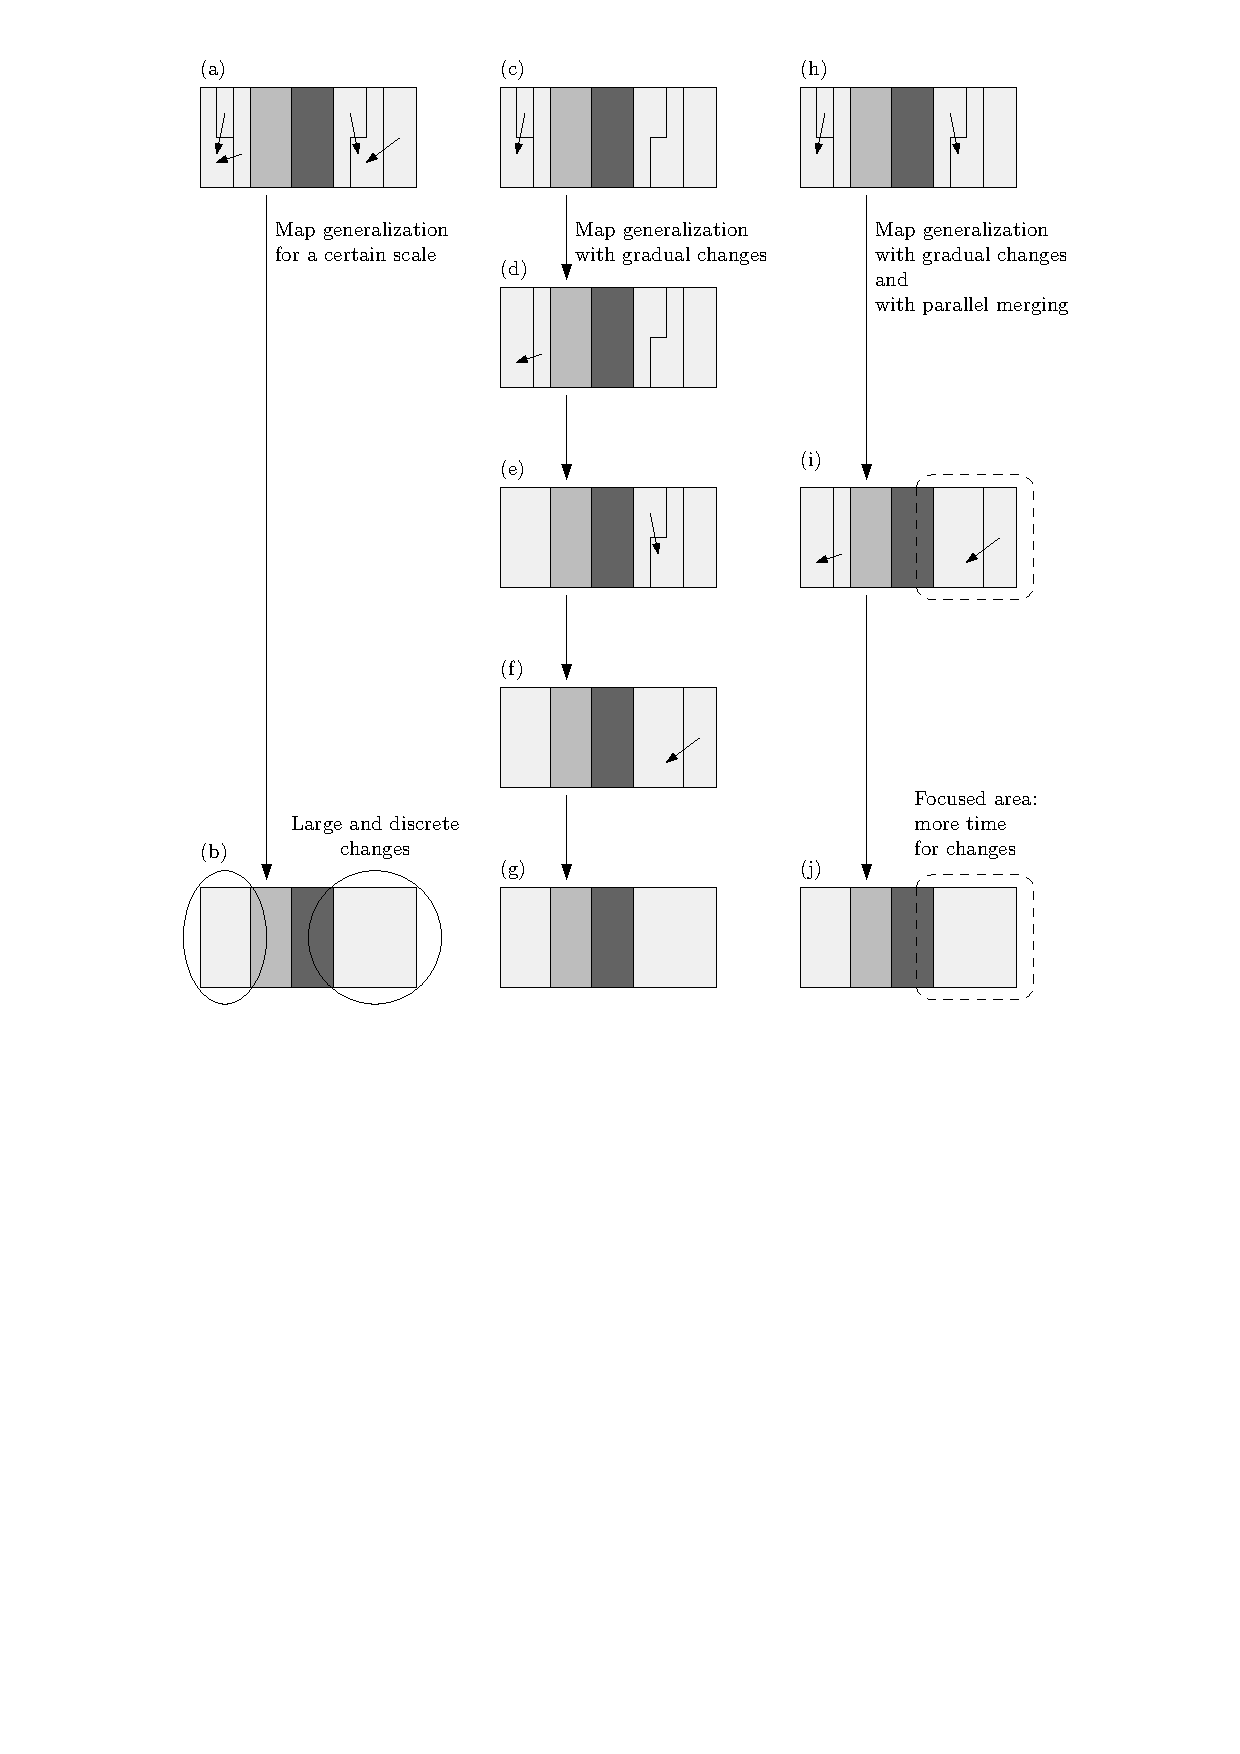
\includegraphics[page=1]{introduction}
\caption{A comparison of different animation strategies for zooming out.
Each arrow inside the subfigures indicates that 
an area will be merged into another one.
The arrow in the right-hand side indicates the animation time of zooming out.
%
(a--c): All changes are processed in one go.
(d--j): All changes are rapidly sequenced one by one.
(k--o): Changes are grouped, resulting in more animation time for every change.
%where smooth and parallel changes going on can be found in figure~(r);
%digital map with smooth and parallel generalization operations.
%
The ellipse shows an example place where large and discrete change happens.
The dashed polygon show the place where a user may focus;
in the place, the user has twice of the time to perceive the merging
of figures (k--l),
comparing to the merging of figures (d--f).
The numbers are the face ids, which will be used in \sect\ref{sec:methodology}.
}
\label{fig:intro}
\end{figure}

\begin{figure}
\centering
\begin{subfigure}[t]{0.48\textwidth}
\centering
\includegraphics[page=4,width=0.95\linewidth]{methodology}
\caption{The SSC of the single-event merging shown in \figs\ref{fig:intro}d--j.
    If slicing the SSC with a horizontal plane at $z$-coordinates~$0$, 
    $100$, $200$, $300$, $400$, $500$, and~$600$,
    then we respectively get \figs\ref{fig:intro}d--j.
    If slicing it at $z$-coordinate~$50$,
    then we get \fig\ref{fig:intro}q.}
\end{subfigure}
\hfill
\begin{subfigure}[t]{0.48\textwidth}
\centering
\includegraphics[page=5,width=0.95\linewidth]{methodology}
\caption{The SSC of the parallel-event merging shown in \figs\ref{fig:intro}k--o.    
    If slicing the SSC with a horizontal plane at $z$-coordinates~$0$, 
    $200$,  $400$, $500$, and~$600$,
    then we respectively get \figs\ref{fig:intro}k--o.
    If slicing it at $z$-coordinate~$100$,
    then we get \fig\ref{fig:intro}r.}
\end{subfigure}
\caption{
The $z$-coordinate corresponds to the denominator of the scale.
The $z$-coordinate also corresponds to the animation time of zooming.
The smooth animation of zooming out can be obtained by
slicing the SSC from bottom to top.
In the SSC, the vertical faces are removed 
because they are not essential for generating a map.
The content of each of the SSCs is stored in an OBJ file,
and each of the figures is generated by displaying the OBJ file
in ParaView~5.8.0.}
\label{fig:ssc_smooth_only}
\end{figure}





When users zoom on maps, 
they do not want to wait for too long to see the desired level.
On a real map, however, 
there are many changes to apply for the scale transition 
when users are zooming out.
If the changes are processed one by one 
(\eg~\figs\ref{fig:intro}d--j),
then the animation time interval for each change has to be very short.
Users may still lose their context 
because it can be difficult for them to perceive necessary changes.
For example, a user may get the impression of
a direct change from \fig\ref{fig:intro}e to \fig\ref{fig:intro}g
(without the intermediate state of \fig\ref{fig:intro}f)
even when the three areas on the right-hand side of \fig\ref{fig:intro}e
are merged gradually as each step is performed very fast.
To provide users with more gradual impression, 
we parallel the generalization operations,
which in this paper are merging operations.
\figs\ref{fig:intro}h--j show such an example,
where at each step two merging operations happen in parallel.
If we select some of the generalization operations
and process them in parallel,
then each operation has more time to take place 
than the operations are processed one after another.\footnote{%
Please try the map at
\url{https://pengdlzn.github.io/webmaps/2020/04/merge-example/paralle-events/}.}
Moreover, if the selected operations
fairly evenly distribute on the whole map, 
then there may be only a limited number of operations 
happening on the screen.
We assume that it is easier for users to follow 
when fewer operations take place longer on the screen.
As for the operations happening outside the screen,
they can be ignored because 
they are not interesting to map users at the moment.
For example, in the focused area, there is only one merging operation 
from \fig\ref{fig:intro}i to \fig\ref{fig:intro}j
while there are two merging operations  
from \fig\ref{fig:intro}e to \fig\ref{fig:intro}g;
a user has twice of the time to perceive the changes of the former,
comparing to the latter.

This paper is organized as follows.
\sect\ref{sec:realted_work} reviews some related work.
Our methodology is presented in \sect\ref{sec:methodology}.
We show a case study in \sect\ref{sec:case_study}.
Finally, \sect\ref{sec:concluding_remarks} draws our conclusion
and present our future work.



 
\section{Related Work}
\label{sec:realted_work}

\Citet{vanOosterom2005} proposed a greedy algorithm 
to merge area objects one by one.
In each iteration, that algorithm takes the least important area and 
merges it into the most compatible neighbor.
The importance of an area is defined 
based on both the size and the classification (class importance).
The compatibility between a pair of areas is defined based on 
both the length of the common boundary and the class similarity
of the two areas. 
\citet[\chap2]{Peng2019Thesis} tried to find an optimal sequence 
to merge area objects
based on the \Astar algorithm or an integer linear program.
A comparison to a greedy algorithm showed that 
the \Astar algorithm improves the quality of the merging sequences
in the sense of the class changes and the compactnesses of the areas.
\Citet{vanOosterom2014Support} pointed out that 
sequentially processing generalization operations 
may result in a suboptimal smooth-zoom effect.
So, they suggested that
the generalization operations should be paralleled.
%Then, one question is how many operations 
%should be paralleled for a given scale.
\citet{Thiemann2018LandCover} proposed a chain of operators 
to generalize a land-cover map.
In the chain of processing area objects, 
they integrated cleaning, dissolving, splitting, aggregating, reclassifying, and simplifying. 

\Citet{vanOosterom2014Support} explained the concept of the space-scale cube (SSC).
At the bottom of the SSC is a detailed land-cover map.
All the area objects extrude along the $z$-axis.
In the SSC, an area on map becomes a polyhedron, and
the common boundary of two areas is a vertical wall.
Whenever a generalization operation happens, 
the extrusions of the involved areas stop;
then, the newly generated areas take the place and start to extrude.
On this basis, the map at any scale can be generated by slicing the SSC 
with a horizontal plane.
That is to say, the scale becomes the third dimension of the map in the SSC
(\eg~\fig\ref{fig:ssc_smooth_only}).
Furthermore, they represented the smooth tGAP in the SSC.
A typical example of the smooth generalization operation is that 
an area merges another one by gradually expanding over it.
In the SSC for the smooth tGAP, 
the wall starts to tilt when the expansion begins.
Based on the SSC, \citet{Meijers2020Web} explained the principles of 
implementing a web map of area objects.
They showed a protocol to react to a map user's browsing the map.
They made chunks of the data used to build the SSC
so that they were able to send only the chunks relevant to the place
where a map user was reading.
They showed how to efficiently slice the SSC to output a web map at a given scale 
using the GPU at the client side.
In addition to slicing the SSC with a horizontal plane,
they could also slice the SSC with a curly surface 
to output a map with mixed scales.
To build the SSC, \citet{Suba2014Merge} proposed three methods 
to merge a pair of areas in a gradual manner, 
which are the ``Single flat plane'', the ``Zipper'', and the ``Eater''.
Basically, the \emph{winner} gradually expands over the \emph{loser}.
We will use the ``Eater'' because it works for all kinds of polygons 
while the other two methods have limitations for some special cases.
\citet{Huang2016Webmap} pointed out that
the effort of implementing online maps 
had been spent mainly on preparing data on the server side.
They studied the communication of map data 
between the server side and the client side.
They proposed different strategies of assigning 
the work of handling map data
according to the machine abilities of the clients.
For example, the two other methods do not work for some concave polygons.


\citet{Suba2016Road} continuously generalized a planar map of road network.
In each step, they process the least important face.
Taking into account the local condition of the face
(\eg~no compatible neighbor at the same side of the road),
they may put it back with higher importance, collapse it, 
or merge it into an adjacent face.
In addition to the generalization, 
they also made statistics of the number of faces,
the area of faces, the number of road faces, the number of road edges,
and the number of operations (merge and split) 
when the scale of the map is decreasing.
These statistics can be good indications 
for (continuous) map generalization.
\citet{Huang2017Matrix} utilized a matrix to guide 
both pruning rivers and removing vertices for a river network, 
where the rows and the columns respectively represent
the rivers and the vertices.
According to the matrix, 
they were able to decide which rivers and vertices 
should be remained for a given scale.
To that purpose, they proposed a method 
to compute how many rivers and vertices 
should be kept according to that given scale.





%\citet{Dumont2020MultiScale}
%\citet{Meijers2015Parallel}

%

\section{Methodology}
\label{sec:methodology}

%UML?
%Flowchart of the framework?

%\subsection{Smooth Merging}
%\label{sec:smooth_merging}

In order to provide smooth merging
so that map users can easily follow the changes,
we merge by gradually expanding an area over another area
(see \fig\ref{fig:intro}q).
%This expansion is based on slicing the space-scale cube (SSC) shown in
%\fig\ref{fig:smooth_merging_ssc}.
%For example, \figs\ref{fig:smooth_merging}a,
%\ref{fig:smooth_merging}b, and \ref{fig:smooth_merging}c
%are respectively obtained from slicing the cube 
%at the bottom, the middle, and the top.
The details of slicing a cube can be found in \citet{Meijers2020Web}.
The SSC of \fig\ref{fig:ssc_smooth_only} was built 
based on the \emph{Eater} of \citet{Suba2014Merge}.
The Eater was used because it provides a solution 
for an area with any kind of shape, which is more robust than
\emph{Single flat plane} and \emph{Zipper} \citep{Suba2014Merge}.
%Note that the common boundary of the two areas disappears
%very shortly after the expansion starts.
%That is, the common boundary exists only in 
%\fig\ref{fig:smooth_merging}a but not in
%\figs\ref{fig:smooth_merging}b,
%\ref{fig:smooth_merging}c, or \ref{fig:smooth_merging}d.


%\begin{figure}[tb]
%\centering
%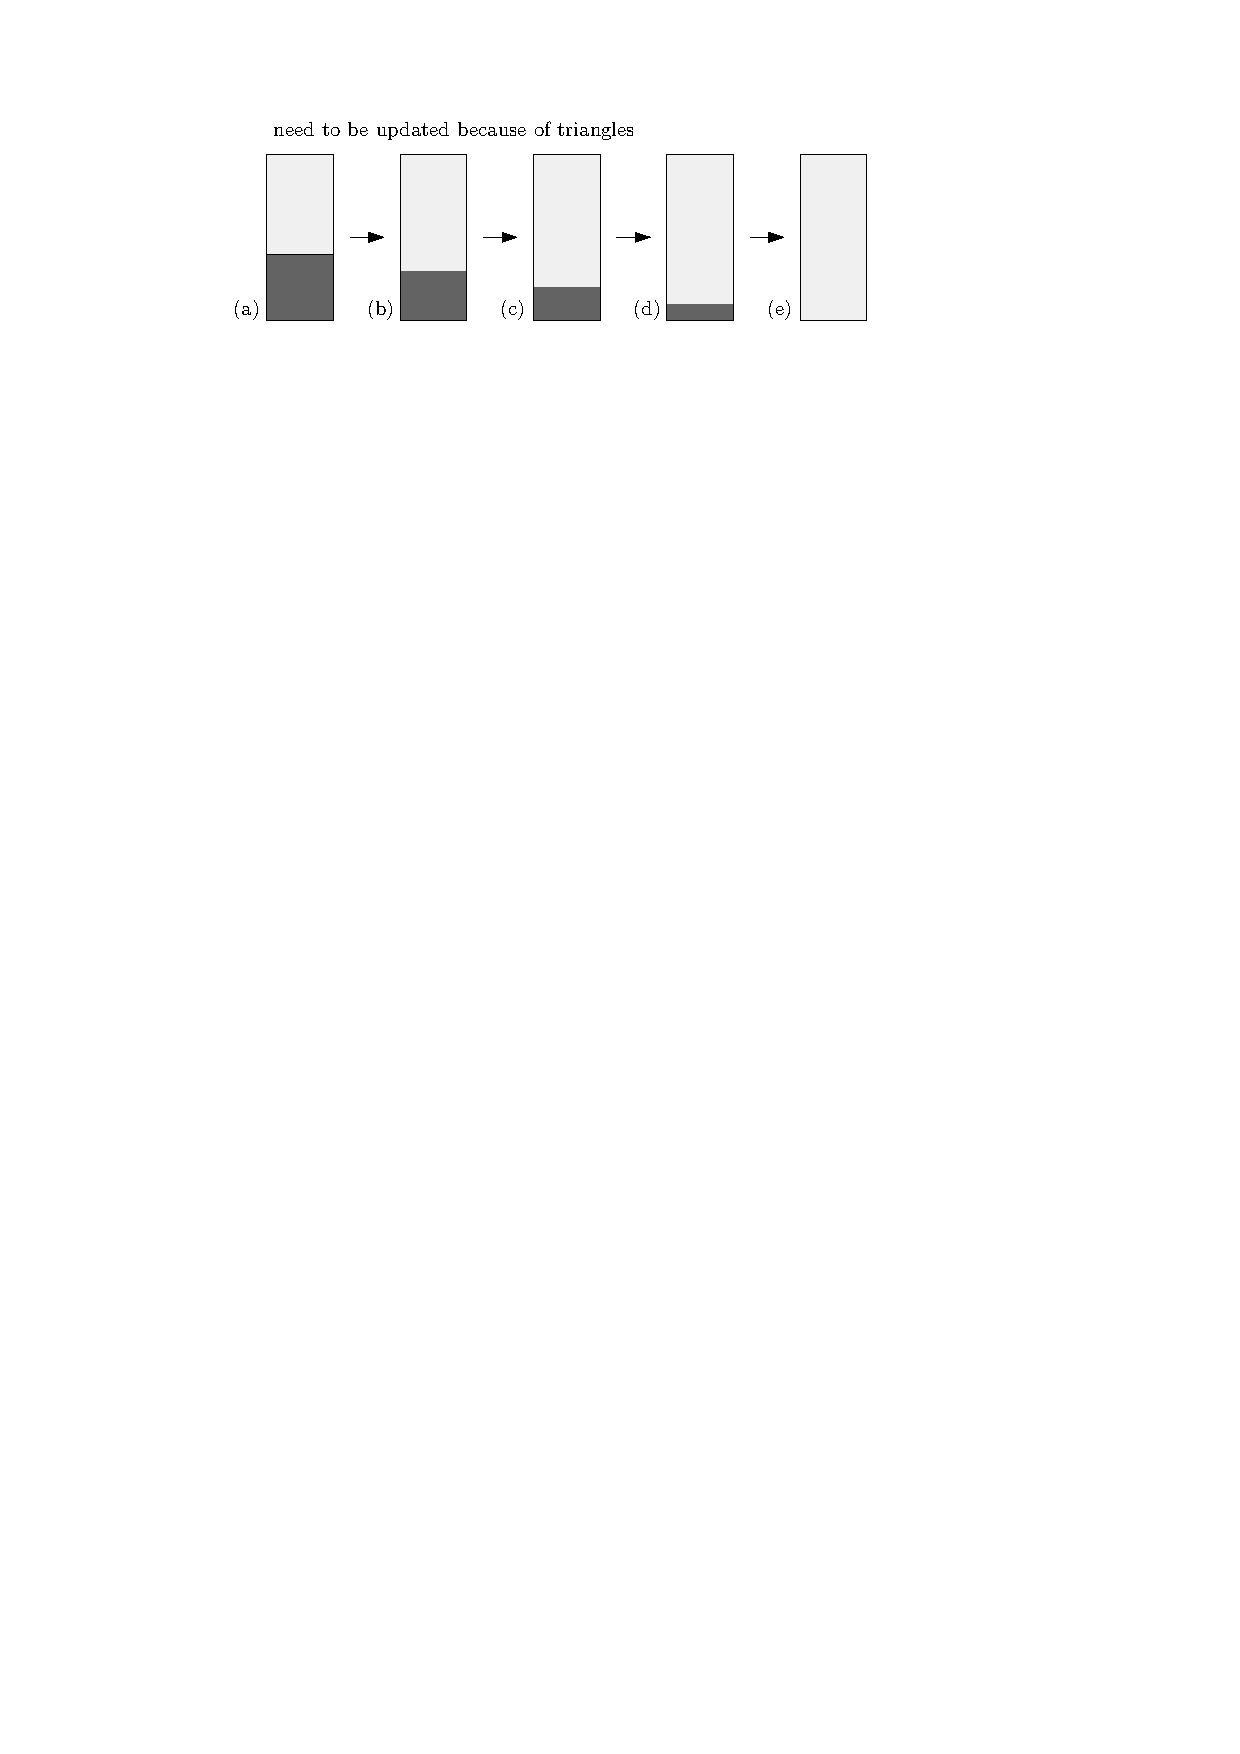
\includegraphics[page=1]{smooth_merging}
%\caption{A smooth way of merging two areas,
%    where the larger area gradually expands over the smaller one.}
%\label{fig:smooth_merging}
%%
%\vspace{6mm}
%%
%\centering
%\includegraphics[page=2, scale=0.3]{smooth_merging}
%\caption{The space-scale cube for the merging 
%    of \fig\ref{fig:smooth_merging}.
%    This figure is made by visualizing the content of an obj file in 
%    ParaView 5.6.0.}
%\label{fig:smooth_merging_ssc}
%\end{figure}


We define an \emph{event} as a single generalization operation, 
such as merging an area into a neighbor.
For example, \fig\ref{fig:intro}e is obtained from 
\fig\ref{fig:intro}d by processing one merging event,
where the arrow in \fig\ref{fig:intro}d indicate the merging.
Similarly, \fig\ref{fig:intro}l is obtained from 
\fig\ref{fig:intro}k by processing two merging events.
We define a \emph{step} as 
a set of events happening at the same time.
For example, 
\fig\ref{fig:intro}e is obtained from 
\fig\ref{fig:intro}d by processing a step with one merging event.
\fig\ref{fig:intro}l is obtained from 
\fig\ref{fig:intro}k by processing a step with two merging events.
In our method, a step is completely processed 
before the next step takes place (all sequential).
We define a \emph{state} as the point when a step starts or finishes.
For example, there are seven states in the merging sequence of \figs\ref{fig:intro}d--j
(\ie~states 0, 1, 2, 3, 4, 5, and 6, from bottom to top)
and five states in the merging sequence of \figs\ref{fig:intro}k--o 
(\ie~states 0, 2, 4, 5, and 6).
The value of a state is also the total number of events processed so far.

%\begin{figure}[tb]
%\centering
%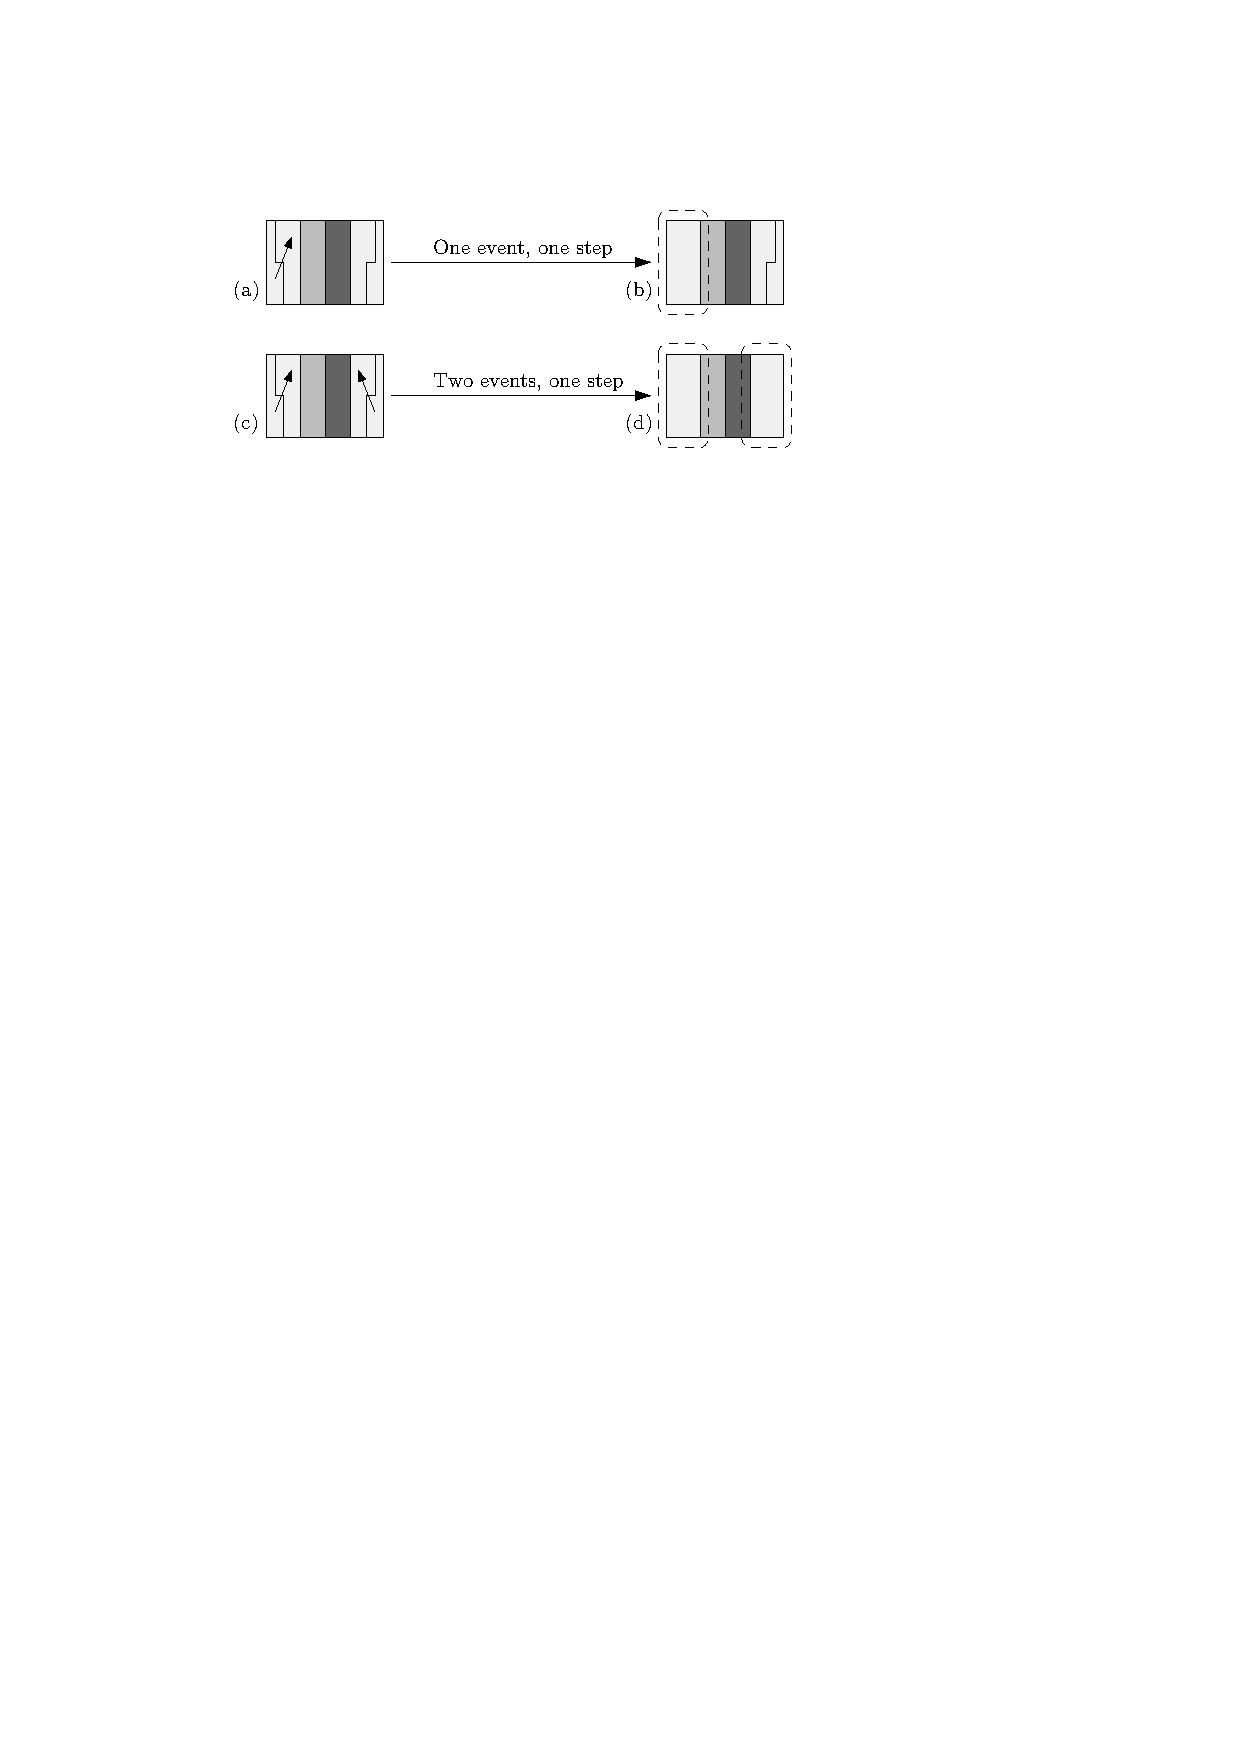
\includegraphics[page=1]{greedy_algorithm}
%\caption{Each path shows a step. 
%A step consists of one or more events (generalization operations).}
%\label{fig:event_and_step}
%\end{figure}


We require that 
the area objects involved in different merging events of the same step 
must not be neighbors, 
which makes the merging events independent from each other.
There are two benefits of this independency.
First, it is easy to maintain the topology of the map.
When a pair of areas have been merged, 
we must update the common boundaries with the surrounding adjacent areas.
If an adjacent area is involved in another merging event,
then it is complicated to update the adjacent area's boundaries
for the two merging events.
Second, users can understand the events more easily 
than merging several areas into a single one,
where the latter is a traditional way of merging.
In order to realize the requirement, during the processing 
we block the neighbors of the areas involved in merging events.
We show a greedy algorithm to find the parallel merging events for each step
in \sect\ref{sec:greedy_algo}.
Then, we integrate the parallel merging events into the tGAP databse tables
(\sect\ref{sec:integrate_tgap}),
followed by integrating the events into the SSC 
(\sect\ref{sec:integrate_ssc}).
In \sect\ref{sec:snap}, we show how to snap the zooming to existing states
to avoid half-way merging animation.

\subsection{A Greedy Algorithm}
\label{sec:greedy_algo}

In the greedy algorithm, we need to obtain the most compatible neighbor 
for a given area.
There are many ways of defining the most compatible neighbor.
For example, \citet{Cheng2006} proposed three ways, i.e.,
the neighbor has the largest size, 
shares the longest boundary with the least important area,
or is has the closest class to the least important area. 
\citet{Peng2017AStar} proposed that 
the most compatible neighbor should have a close classification
to the least important area
and the combination of the two areas should be compact;
they defined the class distance based on a binary tree
according to the codes of the classes.
We currently consider the most compatible neighbor
as the one shares the longest common boundary 
with the least important area,
and we consider the least important area 
as the smallest area on the map.

\fig\ref{fig:greedy_framework} shows the flowchart of our greedy algorithm.
The process starts with state~$s=0$ and a detailed map of area objects, $|M_0|$.
Parallel parameter~$r_\mathrm{parallel}$ specifies 
the proportion of area objects that
we expect to merge parallelly.
Apparently, there holds~$r_\mathrm{parallel} \in (0,1)$.
Expression~$|M_s|$ denotes the number of area objects of the map at state~$s$.
If there is more than one area ($|M_s|>1$),
then we can start to find merging events.
We first compute the number of areas that we expect to merge by
\begin{equation}
\label{eq:n_target}
n_\mathrm{target} =
\lceil r_\mathrm{parallel} \cdot |M_s| \rceil,
\end{equation}
where the ceiling function guarantees~$n_\mathrm{target}\ge 1$.
That is to say, we need to find at least one event for each step.
When~$n_\mathrm{target} > 1$, however,
we cannot always find~$n_\mathrm{target}$ events
because some areas may be blocked as explained before
(also see \fig\ref{fig:blocked_polygons}).
Therefore, we use variable~$n_\mathrm{event}$
to represent the number of events that actually happened within the step. 


\begin{figure}[tb]
\centering
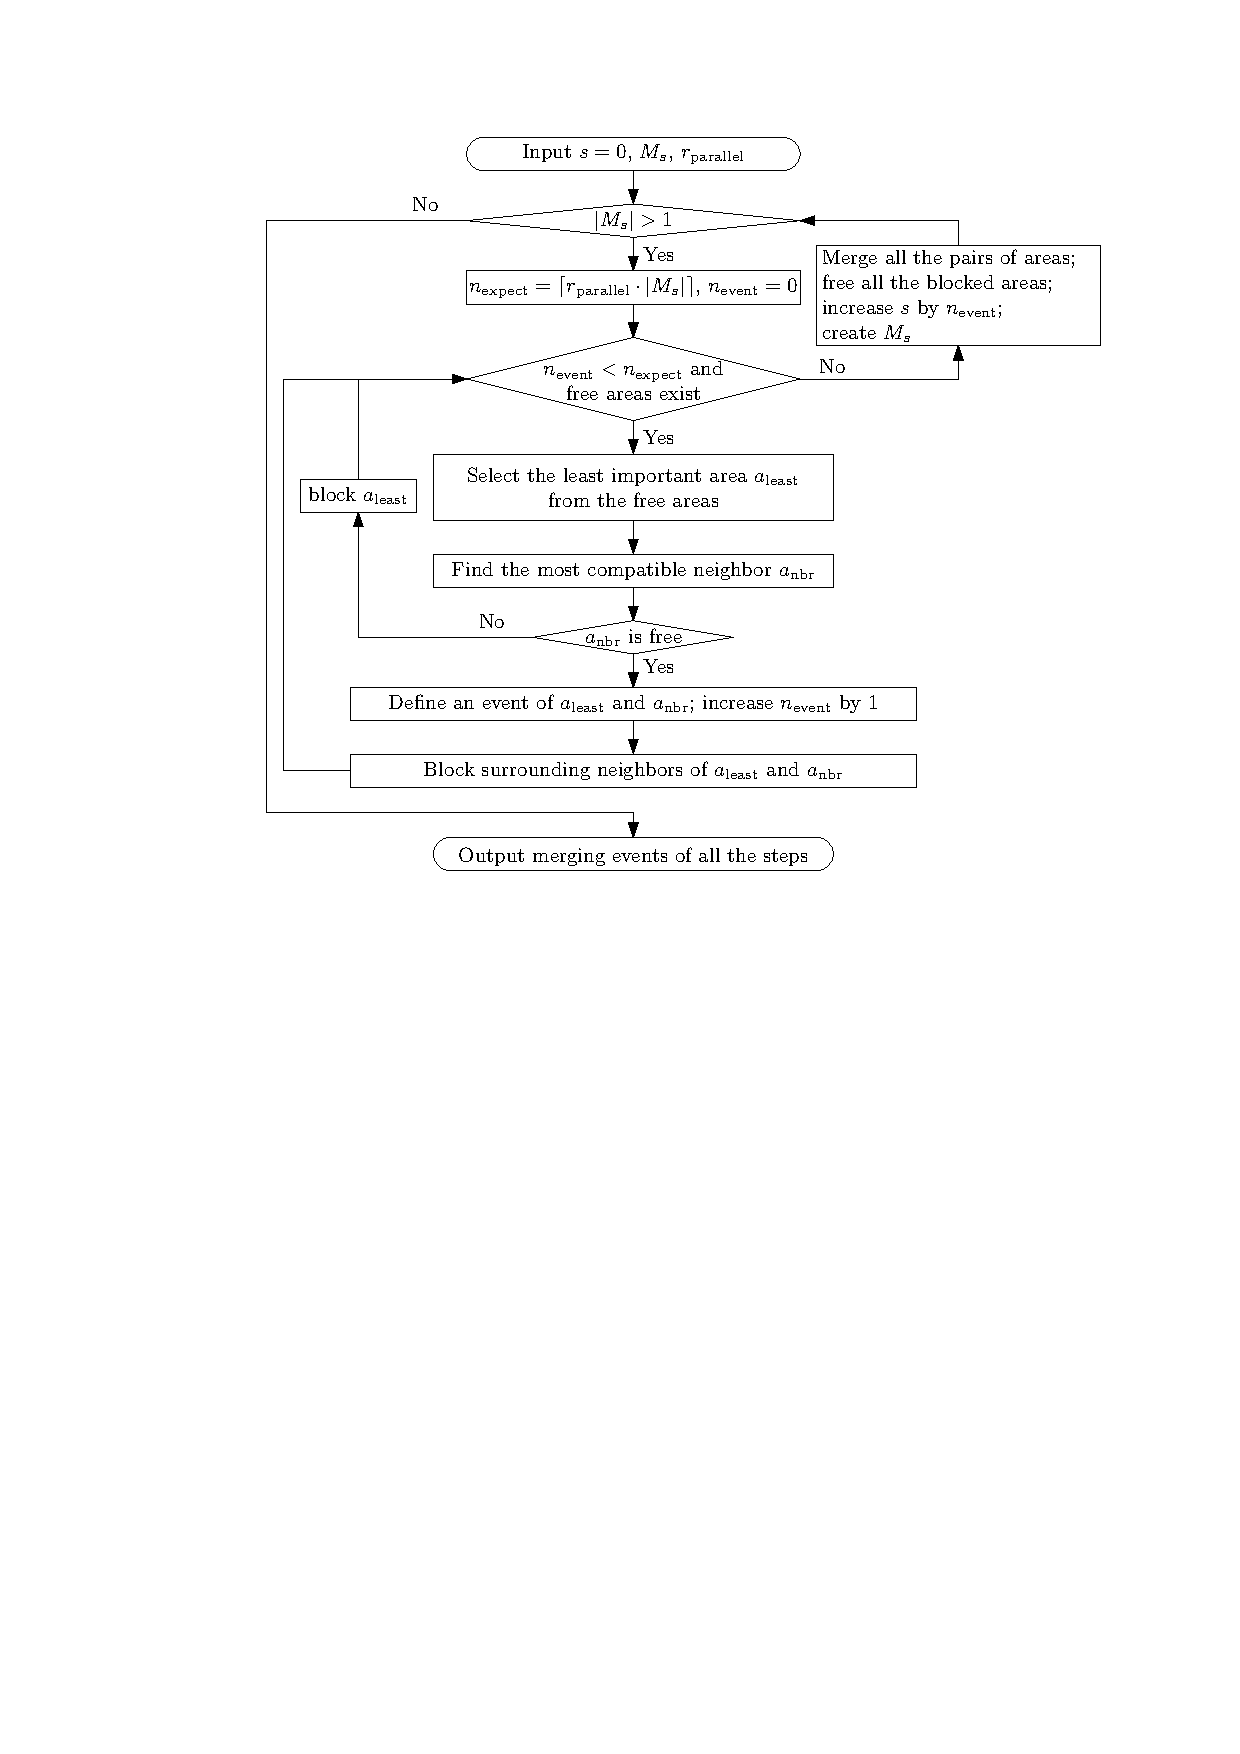
\includegraphics[page=1]{methodology}
\caption{The flowchart of our greedy algorithm.
}
\label{fig:greedy_framework}
\end{figure}


\begin{figure}[tb]
\centering
\includegraphics[page=2]{methodology}
\caption{The process of finding parallel merging events for a step.
    (a) From all the free areas,
	the least important one (the smallest one) is selected to merge into
	its most compatible neighbor (the one shares the longest common boundary).
    The arrow indicates the merging.
	Then the surrounding areas are blocked (marked by the cross).
    Note that the area shares only a vertex with the least important area 
    does not need to be blocked.
	(b) Next, the least important area from the remaining free areas
	is selected to merge with the most compatible neighbor
	(the arrow indicates the merging),
	and the surrounding areas are also blocked.
}
\label{fig:blocked_polygons}
\end{figure}

If we have not found $n_\mathrm{target}$ events 
($n_\mathrm{event} < n_\mathrm{target}$)
and there are still free areas,
then we go on looking for merging events.
An area is \emph{free} if 
it is not involved in an event and is not blocked.
We select the least important area~$a_\mathrm{least}$
from the set of free areas.
We also obtain $a_\mathrm{least}$'s 
most compatible neighbor~$a_\mathrm{nbr}$.
If area~$a_\mathrm{nbr}$ is also free, 
we define an event of areas~$a_\mathrm{least}$ and~$a_\mathrm{nbr}$,
and increase the number of events, $n_\mathrm{event}$, by 1.
We also block the surrounding neighbors of $a_\mathrm{least}$ and $a_\mathrm{nbr}$
(see \fig\ref{fig:blocked_polygons}a).
Then, we continue to find more merging events
(see \fig\ref{fig:blocked_polygons}b).
If area~$a_\mathrm{nbr}$ is not free,
then it must be blocked because of the previously found events.
In this case, we block $a_\mathrm{least}$ for now
so that areas~$a_\mathrm{least}$ and~$a_\mathrm{nbr}$ 
may merge in the next step.

If we have found~$n_\mathrm{target}$ events 
or there is no free area anymore,
then finding merging events of the step finishes.
We parallelly merge all the pairs of areas of the events,
free all the blocked areas,
increase state~$s$ by value~$n_\mathrm{event}$,
and create map~$M_s$ based on the new areas and the freed areas.
Then, finding merging events for the next step starts.
This interation of finding completes 
until there is only one area left on the map ($|M_s|=1$).
The merging events will be stored as records in tGAP database tables
(see \fig\ref{fig:uml_tgap}).
\figs\ref{fig:intro}k--o show a sequence of four merging steps
obtained by our greedy algorithm,
where parallel parameter~$r_\mathrm{parallel}$ is set to~$0.3$
(Note that this is an extremely high value, 
just used to explain the principle in an artificial simple example).



\begin{figure}[tb]
\centering
\includegraphics[page=3]{methodology}
\caption{The UML diagram of the classes stored in tGAP databse tables.
This diagram is a slightly improved version of \citet[\p159]{Meijers2011Thesis}.
In the face table, property \emph{pip\_geometry} 
stores a point (usually the center) in the face (polygon).
The geometry of a face can be obtained by calling function \emph{getGeometry()}.
We do not store the face geometry because we want to avoid redundancy,
as the edges already stores sequences of points.
}
\label{fig:uml_tgap}
\end{figure}



%\begin{figure}[tb]
%\centering
%\includegraphics[page=2]{blocked_polygons}
%\caption{A sequence of merging steps obtained by our greedy algorithm,
%	where parallel parameter~$r_\mathrm{parallel}$ is set to~$0.3$.
%    Note that~$\mathrm{state}=1$ does not exist in this merging sequence
%    while step number increases by~$1$ each time.
%	The arrows in the subfigures indicate merging events.
%}
%\label{fig:sequence_greedy}
%\end{figure}





\subsection{Integrating the parallel events into the tGAP Databse Tables}
\label{sec:integrate_tgap}

\citet[\p159]{Meijers2011Thesis} designed three tables 
to record the information of
faces, edges, and face hierarchies, 
which together form a tGAP.
For example, the face table contains columns \emph{face\_id}, 
\emph{imp\_low}, \emph{imp\_high}, \emph{imp\_own},
\emph{feature\_class}, \emph{area}, and \emph{mbr\_geometry}.
We add columns \emph{state\_low} and \emph{state\_high} into the table 
so that it is easy to see when a face should appear or disappear 
(see \tbls\ref{tbl:face_tgap}a and~\ref{tbl:face_tgap}b,
where all other columns, except face\_id, are hidden).
When the map is zoomed out, a face should appear
when the slicing arrives at the state\_low value,
and the face should disappear
when the slicing arrives at the state\_high value.
Comparing between the tables of single-event merging 
(\figs\ref{fig:intro}d--j)
and parallel-event merging (\figs\ref{fig:intro}k--o),
we observed some differences.
For example, the state\_high values of faces~1 and~2 are changed from~1 to~2
(see \tbl\ref{tbl:face_tgap}).
Also, the state\_low value of face~8 is changed from~1 to~2
(see \tbl\ref{tbl:face_tgap}).
The columns and records of both the edge table and the face-hierarchy table 
will be changed accordingly.


\begin{table}[tb]
\caption{Some columns of the face tables. 
In table~(b), the different values from table~(a) are underlined.}
\label{tbl:face_tgap}
\begin{subtable}{0.45\textwidth}
\caption{The face table of the single-event merging 
    shown in \figs\ref{fig:intro}d--j.}
\centering
\begin{tabular}{ccc}
\toprule
face\_id & state\_low   & state\_high \\ \midrule
1       &     0         &     1       \\
2       &     0         &     1       \\
3       &     0         &     2       \\ 
4       &     0         &     5       \\
5       &     0         &     4       \\
6       &     0         &     3       \\         
7       &     0         &     3       \\
8       &     1         &     2       \\
9       &     2         &     6       \\         
10      &     3         &     4       \\
11      &     4         &     5       \\ 
12      &     5         &     6       \\ 
13      &     6         &    ---      \\
\bottomrule
\end{tabular}
\end{subtable}
%
\hfill
%
\begin{subtable}{0.45\textwidth}
\caption{The face table of the parallel-event merging 
    shown in \figs\ref{fig:intro}k--o.}
\centering
\begin{tabular}{ccc} %\underbar{2}
\toprule
face\_id & state\_low   & state\_high \\ \midrule
1       &     0         &\underbar{2} \\
2       &     0         &\underbar{2} \\
3       &     0         &\underbar{4} \\ 
4       &     0         &     5       \\
5       &     0         &     4       \\
6       &     0         &\underbar{2} \\         
7       &     0         &\underbar{2} \\
8       &\underbar{2}   &\underbar{4} \\
9       &     2         &\underbar{6} \\         
10      &\underbar{4}   &\underbar{4} \\
11      &     4         &     5       \\ 
12      &     5         &     6       \\ 
13      &     6         &    ---      \\
\bottomrule
\end{tabular}
\end{subtable}
\end{table}



\subsection{Integrating the parallel events into the SSC}
\label{sec:integrate_ssc}

Recall that we merge a pair of areas by expanding one over 
the less important one.
The Eater of \citet{Suba2014Merge} is used to 
triangulate the less important area and to tilt the triangles.
Then the tilted triangles are integrated into the SSC
(see \fig\ref{fig:ssc_smooth_only})
so that we can slice the SSC to achieve smooth merging.
For the case of single-event merging,
if a pair of areas have state\_high value~$s_\mathrm{high}$,
then the merging animation 
always starts at state~$s_\mathrm{expand}=s_\mathrm{high}-1$.
The less important area completely disappears
at state~$s_\mathrm{high}$.
In the face table, a row will be added 
to record the new area, and its state\_low value will be~$s_\mathrm{high}$.
The new area takes the combined place of the pair of areas.
Take \ref{fig:intro} as an example, 
area~1 is merged into area~2 (\figs\ref{fig:intro}d), 
and area~8 is generated to take the combined place (\figs\ref{fig:intro}e).
The tilted triangle is the one spans 
from $z= 0$ to $z=100$ (\ie~from state~0 to state~1)
in \fig\ref{fig:ssc_smooth_only}a.
In \tbl\ref{tbl:face_tgap}a, we see that
the state\_low value of area~8 is 1,
which is the state\_high value of areas~1 and~2.
Note that the state\_low values of the two areas do not matter 
because those values respectively indicate the states that
the two areas appear;
those values can be much smaller 
than value~$s_\mathrm{high}-1$.

For the case of parallel-event merging,
if a step consists of~$n_\mathrm{event}$ events and 
the step finishes at state~$s_\mathrm{high}$, then the step starts 
at state~$s_\mathrm{expand}=s_\mathrm{high} - n_\mathrm{event}$.
The reason is that if the $n_\mathrm{event}$ events 
would happen sequentially (\ie~single-event merging),
then they would take place 
from state~$s_\mathrm{high} - n_\mathrm{event}$ to state~$s_\mathrm{high}$.
When all the events take place parallelly in the same step, 
each of the events can share
its time duration of expansion animation.
%there is a less important area in each of the parallel events of a merging step.
%If the number of parallel events is~$n_\mathrm{event}$,
%then there are~$2n_\mathrm{event}$ areas 
%with the same state\_high value, say,~$s_\mathrm{high}$
%because each merging event involves two areas.
%The merging animations of all the parallel events
%start at state~$s_\mathrm{expand}=s_\mathrm{high} - n_\mathrm{event}$
%and finishes at state~$s_\mathrm{high}$.
%By definition, the parallel events of a merging step 
%happen during the same animation time.
%In other words, the areas involved in those parallel events have 
%the same state\_expand value ($s_\mathrm{expand}$) and 
%the same state\_high value ($s_\mathrm{high}$).
%The reverse is also true.
%If some areas have the same state\_high value,
%then those areas happen during the same animation time 
%(involved in the parallel events of the same step).
%The reason is that, according to our requirement,
%a step can start only when the previous step stops.
%Thus, the merging events finishing at the same state cannot from different steps.
%of these areas 
%will finish at state~$s_\mathrm{high}$,
%and no merging event will start earlier or later than state~$s_\mathrm{expand}$
%because we required that the next step starts only when a step stops.
Given the fact that the animation time for zooming 
between state~$s_\mathrm{expand}$ and state~$s_\mathrm{high}$ is fixed,
each of the parallel events has more time to take place
than the events would happen sequentially.
In other words, for a merging step finishes at state~$s_\mathrm{high}$,
each of the events of the step has more time to take place 
if there are more events happen parallelly.

In order to build the SSC for parallel merging,
we need the~$s_\mathrm{expand}$ value for each of the merging steps
so that we know at which state 
the triangles of the less important areas should be tilted.
A simple way is to add a column, say, \emph{state\_expand} 
into the face table during generating the tGAP.
Then, the states of starting expansion can be recorded into the column.
However, we would like to avoid unnecessary columns
so that the table is concise and easy to read.
Therefore, we compute state\_expand values 
based on the state\_high values
on the fly when building the SSC.
As an event involves two areas,
the number of events finishing at state~$s_\mathrm{high}$ can be calculated by
\begin{equation}
\label{eq:n_event_state}
n_\mathrm{event} (s_\mathrm{high}) = 
\frac{\sum\limits_{s \in S_\mathrm{high}} [s=s_\mathrm{high}]}{2},
\end{equation}
where notation~$S_\mathrm{high}$ denotes the set of values
recorded in column state\_high of the face table
(\eg~\tbl\ref{tbl:face_tgap}b),
and expression~$[s=s_\mathrm{high}]$ returns~$1$ if the two values are equal 
and returns~$0$ otherwise.
As illustrated before, the state at which the parallel merging animations start 
can be computed by
\begin{equation}
\label{eq:s_expand_state}
s_\mathrm{expand} (s_\mathrm{high}) = s_\mathrm{high} - n_\mathrm{event} (s_\mathrm{high}).
\end{equation}



Take the case of \tbl\ref{tbl:face_tgap}b for example,
we have~$S_\mathrm{end} = \{2, 2, 4, 5, 4, 2, 2, 4, 6, 4, 5, 6\}$, 
$n_\mathrm{event} (4) = 2$, and~$s_\mathrm{expand} (4) = 2$.
Therefore, there are two merging events finishing at state~$4$,
\ie~event of merging area 3 into area~8 and 
event of merging area~5 into area~10 
(also see \figs\ref{fig:intro}l and~\ref{fig:intro}m).
The merging animation takes place from state~$2$ to state~$4$.
This merging can be also observed from 
the two tilted faces above the two light-yellow faces 
in \fig\ref{fig:ssc_smooth_only}b.
In merging sequence of \figs\ref{fig:intro}d--j, 
the animation of merging area~3 into area~8 
takes place from state~$1$ to state~$2$
(also see the tilted face above the light-yellow face 
on the left-hand side of \fig\ref{fig:ssc_smooth_only}a), and 
the animation of merging area~5 into area~10
takes place from state~$3$ to state~$4$
(see the tilted face above the light-yellow face 
on the right-hand side of \fig\ref{fig:ssc_smooth_only}a).
As a result, the animation duration of merging area~3 into area~8 of 
sequence \figs\ref{fig:intro}k--o
is almost twice as that of sequence \figs\ref{fig:intro}d--j.
We say \emph{almost} because the animation duration is also dependent on 
which state we are at 
\textbf{see section of relationship between time duration and time}.


%According to \tbl\ref{tbl:face_tgap}, 
%face~1 and face~2 are merged from state~0 to state~1,
%which is before the merging of face~5 and face~6 from state~1 to state~2.
%According to \tbl\ref{tbl:face_tgap}b, 
%the merging of face~1 and face~2 and the merging of face~5 and face~6
%happen parallelly from state~0 to state~2.
%
%Then, the space-scale cube will be built 
%according to the records of \tbl\ref{tbl:face_tgap}b.









\subsection{Snapping to an Existing State}
\label{sec:snap}

When at the client side 
using the SCC with parallel events for a zooming action
(that is, slicing the SSC with a horizontal plane), 
we always snap the map to an existing state.
In this way, users will not see a merging operation stops half-way
and will not see transition artifact (such as slivers).
Take the sequence of \fig\ref{fig:intro}k--o for example, 
the merging animation should stop at 
either \ref{fig:intro}k or \ref{fig:intro}l,
but not at \ref{fig:intro}r.
%Note that some states do not exist because of the parallel events.
%For example, state~$1$ does not exist 
%in the sequence of \fig\ref{fig:intro}k--o.
%In such case, the merging animation should not stop at state~$1$.
In order to snap to existing states,
we have to communicate the valid states to the client side. 
There are multiple options. 
The most simple one assumes that, 
during the creation of the parallel SCC, 
we can always perform the~$n_\mathrm{target}$ number of events in all steps. 
In that case, we just have to communicate 
the number of areas and the ratio~$r_\mathrm{parallel}$. 
In case of high value ratios ($> 0.01$), 
this assumption may not be correct. 
We then have to communicate the valid states by sending them explicitly. 
Because this list may get rather large,
we compress the information of merging events and save it into 
a JSON file (JavaScript Object Notation File).
Then, the JSON file will be sent to the client side and uncompressed.


\subsubsection{On the Server Side}
\label{sec:snap_server}

On the server side, we compute the values shown in \tbl\ref{tbl:sequence_greedy}.
\tbl\ref{tbl:sequence_greedy} is based on the merging steps of
\fig\ref{fig:intro}k--o,
where parallel parameter~$r_\mathrm{parallel}$ is set to~$0.3$.
Note this value is extremely high, 
just used to explain the principle in an artificial simple example.
The computation starts from step~$1$.
At the beginning, there are $7$ areas on the map, \ie~$|M_0| = 7$.
According to \eq\ref{eq:n_target},
we expect to parallel three events ($n_{\mathrm{target},1} = 3$).
However, only two event can be paralleled in step~$1$ 
according to the situation of \fig\ref{fig:intro}k.
Therefore, we have~$n_{\mathrm{event},1} = 2$.
The difference of the expected value and the real value
can be computed by
\begin{equation}
\label{eq:n_diff}
n_{\mathrm{diff},i} = n_{\mathrm{target},i} - n_{\mathrm{event},i},
\end{equation}
where variable~$i$ indicates the $i$-th step.
That is, we have~$n_{\mathrm{diff},1}=1$, for step~$1$
(also see the $n_\mathrm{diff}$ value in the first row of \tbl\ref{tbl:sequence_greedy}).
We require that the low state is~$s_{\mathrm{low},1} = 0$ for the first step.
Then, the state\_high value can be computed by
\begin{equation}
\label{eq:state_high}
s_{\mathrm{high},i} = s_{\mathrm{low},i} + n_{\mathrm{event},i}.
\end{equation}
That is, we have~$s_{\mathrm{high},1}=2$
(also see the state\_high value in the first row of \tbl\ref{tbl:sequence_greedy}).
At this point, the computation for step~$1$ completes.


\begin{figure}[tb]
%\centering
%\includegraphics[page=2]{blocked_polygons}
%\caption{.
%}
%\label{fig:sequence_greedy}
%\vspace{6mm} %for some reason, the space below the caption is not enough
%
%
%
\captionsetup*{type=table} %*: suppress warning "The caption type was already set to figure"
\caption{Some information of the merging sequence shown in \tbl\ref{tbl:sequence_greedy}.
Column~$n_\mathrm{area}$ shows the area number of the map at starting state~$s$,
that is, $|M_s|$ of \eq\ref{eq:n_target}.
}
\label{tbl:sequence_greedy}
\centering
\begin{tabular}{ccccccc}
\toprule
step & $n_\mathrm{area}$ & $n_\mathrm{target}$ 
& $n_\mathrm{event}$ & $n_\mathrm{diff}$ & state\_low & state\_high \\ \midrule
1        & 7      & 3        & 2        & 1     & 0      & 2      \\
2        & 5      & 2        & 2        & 0     & 2      & 4      \\
3        & 3      & 1        & 1        & 0     & 4      & 5      \\
4        & 2      & 1        & 1        & 0     & 5      & 6      \\
%5        & 2      & 1        & 1        & 0     & 5      & 6      \\
%6     & 1      & ---      & ---      & ---    \\ 
\bottomrule
\end{tabular}
\end{figure}

For the next step, the number of areas can be computed by
$$
n_{\mathrm{area},i+1} = n_{\mathrm{area},i} - n_{\mathrm{event},i},
$$
where variable~$n_{\mathrm{area},i}$ denotes the area number 
at the low state of step~$i$.
Furthermore, the state\_low value, $s_{\mathrm{low},i+1}$, is the same as  
$s_{\mathrm{high},i}$.
Again, the target number of parallel events, $n_{\mathrm{target},i+1}$,
can be computed by \eq\ref{eq:n_target},
the number of actual parallel events can be obtained from the greedy algorithm,
the value of difference, $n_{\mathrm{diff},i+1}$, 
can be computed by \eq\ref{eq:n_diff}, 
and the state\_high value, $s_{\mathrm{high},i+1}$, 
can be computed by \eq\ref{eq:state_high}.
The computation of all the steps starts from step~$i=1$ and 
finishes until only one area left on the map.
As a result, we have all the values of \tbl\ref{tbl:sequence_greedy}.


%Then the difference in step~$i$ is
%\begin{equation}
%\label{eq:n_diff}
%n_{\mathrm{diff},i} = n_{\mathrm{target},i} - n_{\mathrm{event},i},
%\end{equation}
%where variables~$n_{\mathrm{target},i}$ and~$n_{\mathrm{event},i}$
%are respectively the expected and the real numbers of events in step~$i$,
%which are consistent with the definitions of 
%\eqs\ref{eq:n_target} and~\ref{eq:n_event_state}.
%For the next step, we compute
%$$
%n_{\mathrm{area},i+1} = n_{\mathrm{area},i} - n_{\mathrm{event},i},
%$$
%where variable~$n_{\mathrm{area},i}$
%represents the area number at the starting state of step~$i$.
%Based on number~$n_{\mathrm{area},i+1}$,
%we can further compute $n_{\mathrm{target},i+1}$ and obtain $n_{\mathrm{event},i+1}$.
%This process starts from step~$i=1$ and ends until only one area left.

Now, we have a column of $n_\mathrm{diff}$ values.
Among them, we record the non-zero values and the corresponding steps in a list.
Take \tbl\ref{tbl:sequence_greedy} for example,
the list is $[[1, 1]]$.
The content of the JSON file is as following.
\begin{verbatim}
                {
                    "face_num": 7,
                    "parallel_param": 0.3,                    
                    "step_eventdiff": [[1, 1]]
                }
\end{verbatim}


%We compress those values as the form of 
%$$
%[[n_{\mathrm{diff},1},j_1], [n_{\mathrm{diff},1+j_1},j_2], \ldots, 
%[n_{\mathrm{diff},i},j_k], [n_{\mathrm{diff},i+j_k},j_{k+1}], \ldots],
%$$
%where variable~$j_k$ is the number of the same $n_\mathrm{diff}$ values in a row 
%starting at step~$i$.
%Take \tbl\ref{tbl:sequence_greedy} for example, 
%the value of~$j_1$ is~$1$
%because the following value (\ie~0) is already different 
%from the first value (\ie~1) of~$n_\mathrm{diff}$.
%The value of~$j_2$ is~$3$ 
%because there are three same values in a row (\ie~0). 
%According to our strategy, 
%the~$n_\mathrm{diff}$ values of \tbl\ref{tbl:sequence_greedy}
%will be compressed to~$[[1,1], [0,3]]$,
%where each pair of values in the inner square brackets 
%record an~$n_\mathrm{diff}$ value and the number of repeat times.
%The content of the JSON file is as following.
%\begin{verbatim}
%                {
%                    "face_num": 7,
%                    "parallel_param": 0.3,                    
%                    "step_eventdiff": [[1, 1]]
%                }
%\end{verbatim}
%If we would have a list of $n_\mathrm{diff}$ values~$[0, 0, 0, 0, 0, 0, 5, 0, 0]$,
%then the compressed content would be~$[[0,6], [5,1], [0,2]]$.
%Our case study will show that this way of compressing is efficient
%(see \sect\ref{sec:case_study}).



\subsubsection{On the Client Side}
\label{sec:snap_client}


When a user opens our web map,
the JSON file will be sent to the client side.
We can unpack the content of entry ``step\_eventdiff'' and 
get the list of $n_\mathrm{diff}$ values~$[1, 0, 0, 0]$.
Starting from step~$i=1$,
we can again compute~$n_{\mathrm{target},i}$ according to \eq\ref{eq:n_target},
where parallel parameter~$r_\mathrm{parallel}=0.3$ 
and face number~$n_{\mathrm{area},1} = 7$
can be obtained also from the JSON file.
Then, we can compute the actual number of parallel events by
\begin{equation*}
\label{eq:n_event_step}
n_{\mathrm{event},i} = n_{\mathrm{target},i} - n_{\mathrm{diff},i},
\end{equation*}
which is an inverse function of \eq\ref{eq:n_diff}.
The computed~$n_\mathrm{event}$ values 
should be the same as the values before compressing
(see column~$n_\mathrm{event}$ in \tbl\ref{tbl:sequence_greedy}).

According to the~$n_\mathrm{event}$ values,
we can compute the accumulated number of events~$L_\mathrm{event} = 
[0, 2, 4, 5, 6]$,
which is also the list of existing states
(see columns~state\_low and state\_high in \tbl\ref{tbl:sequence_greedy}).
According to how much a user has zoomed,
a scale, say, $1:S_t$ can be computed.
%According to \citet{Huang2016Webmap},
%the number of merging events that should be processed can be computed by
\citet{Huang2016Webmap} suggested that 
the average density of areas over the whole domain
on a screen should be remained for zooming.
Their suggestion is based on the assumption that 
the area density of the base map is well designed, which is reasonable.
We use variable~$A_\mathrm{real}$ to denote the total areal size of 
all the area objects in reality.
Then, the size on screen at scale~$S_t$ 
is~$A_\mathrm{real} \big/ S_t$,
where~$1:S^2_t$ is the scale that we want to zoom to.
In order to keep the density, we require
\begin{equation}
\label{eq:equal_density}
\frac{N_b}{A_\mathrm{real} \big/ S^2_b} =
\frac{N_b-E_t}{A_\mathrm{real} \big/ S^2_t},
\end{equation}
where parameter~$N_b = |M_0|$ is the number of area objects on the base map,
parameter~$S_b$ is the scale denominator of the base map,
and variable~$E_t$ is the total number of events 
happening from the base map to the map at scale~$1:S_t$.
\eq\ref{eq:equal_density} yields
\begin{equation}
\label{eq:E_t}
E_t = N_b \left(1-\frac{S^2_b}{S^2_t}\right),
\end{equation}
In our example regarding to list~$L_\mathrm{event}$,
if event number~$E_t \le 0$, the base map should be presented;
if $E_t \ge 6$, the last value of list~$L_\mathrm{event}$,
the map with the final single area should be presented.
Otherwise, if $0<E_t < 6$, we snap event number~$E_t$ 
to the closest value (measured in events) of list~$L_\mathrm{event}$,
which is denoted by~$E_{t,\mathrm{snap}}$.
The scale denominator corresponding to event number~$E_{t,\mathrm{snap}}$
can be computed by 
\begin{equation}
\label{eq:S_t_snap}
S_{t,\mathrm{snap}} = S_b \sqrt{\frac{N_b}{N_b-E_{t,\mathrm{snap}}}}.
\end{equation}
Note that \eq\ref{eq:S_t_snap} is an inverse function of \eq\ref{eq:E_t}.
At the end of the zooming action, 
the map will snap to state~$E_{t,\mathrm{snap}}$,
which is at scale~$1:S_{t,\mathrm{snap}}$.


%\subsection{Line simplification (smoothly moving vertices for the SSC)}


\section{Case Study}
\label{sec:case_study}

We have stored the result of the tGAP 
as a set of tables (see \sect\ref{sec:integrate_tgap}) 
in the PostgreSQL database.
We have employed the ``Eater'' of \citet{Suba2014Merge},
implemented in Python, 
to generate the elements
(vertices, triangulated faces, and boundaries)
of the SSC \citep{vanOosterom2014tGAPSSC} 
and saved these elements in an OBJ file.\footnote{%
Wavefront .obj file:
\url{https://en.wikipedia.org/wiki/Wavefront_.obj_file},
accessed: Jan 14, 2020.}
%
The OBJ file and the JSON file (described in \sect\ref{sec:snap_server}) 
will be sent to the client 
when a user visits our website to access the map.
On the client side,
the two files are processed
by a prototype implemented in JavaScript.
The processed content and some code for WebGL (Web Graphics Library)
are submitted to GPU to display the map of smooth zoom.


The dataset used in this case study is a topographic map, 
a subset of TOP10NL,
produced by Kadaster.\footnote{%
More information about TOP10NL can be found at
\url{https://zakelijk.kadaster.nl/-/topnl},
accessed: Jan 14, 2020.}
%
\figs\ref{fig:data}a and~\ref{fig:data}c show the map and the legend.\footnote{%
More details about the class code and the rendering formula can be found at
\url{http://register.geostandaarden.nl/visualisatie/top10nl/1.2.0/BRT_TOP10NL_1.2_beschrijving_visualisatie.xlsx},
accessed: Jan 15, 2020.}
%
Because the base scale is $1:10{,}000$, 
we have~$S_b = 10{,}000$ for \eq\ref{eq:S_t_snap}.
The maximum value for event number~$E_{t,\mathrm{snap}}$ is~$13{,}237$
as there are in total~$13{,}238$ areas.
When we zoom out far enough 
so that~$E_{t,\mathrm{snap}}$ reaches its maximum value,
the scale denominator will arrive at~$1{,}150{,}565$
according to \eq\ref{eq:S_t_snap}.
At that moment, all the areas are merged into one single area
(see \figs\ref{fig:data}b).
In each step, we want to parallelly merge some proportion of the areas.
We tried three cases: 0.1\%, 1\%, and 10\%.
That is, parallel parameter~$r_\mathrm{parallel}=0.001, 0.01, \text{and~} 0.1$ 
(see \sect\ref{sec:greedy_algo}).The three versions can be browsed online.\footnote{%
Our web maps can be found at
\url{https://pengdlzn.github.io/webmaps/2020/03/merge/}.} 
\fig\ref{fig:web_map} shows an example of our web map when 
parallel parameter~$r_\mathrm{parallel}=0.01$.
In addition, the version of single-event step is also available online.


\begin{figure}[tb]
\centering
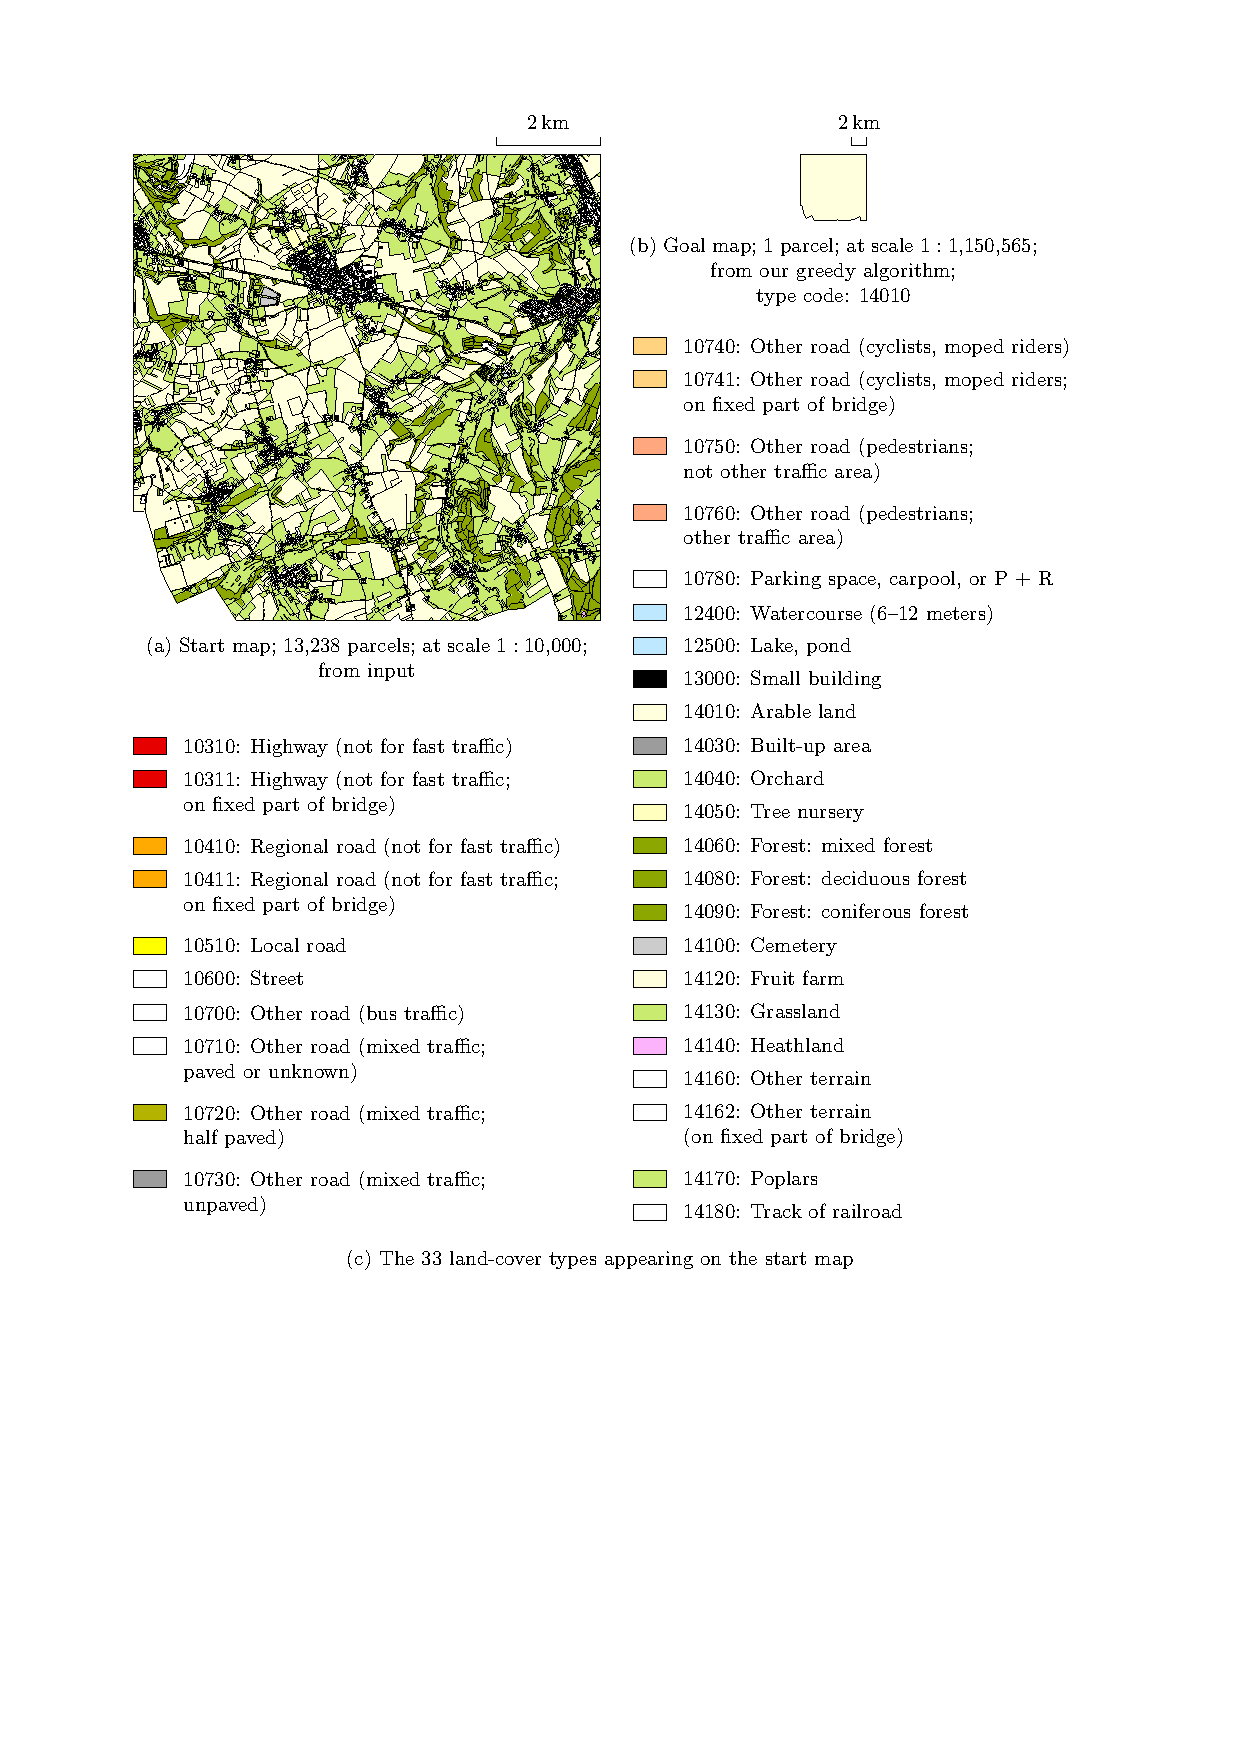
\includegraphics[page=1]{data}
\caption{The topographic map represents the place 
    in the south of Limburg, The Netherlands.}
\label{fig:data}
\end{figure}


\begin{figure}[tb]
\centering
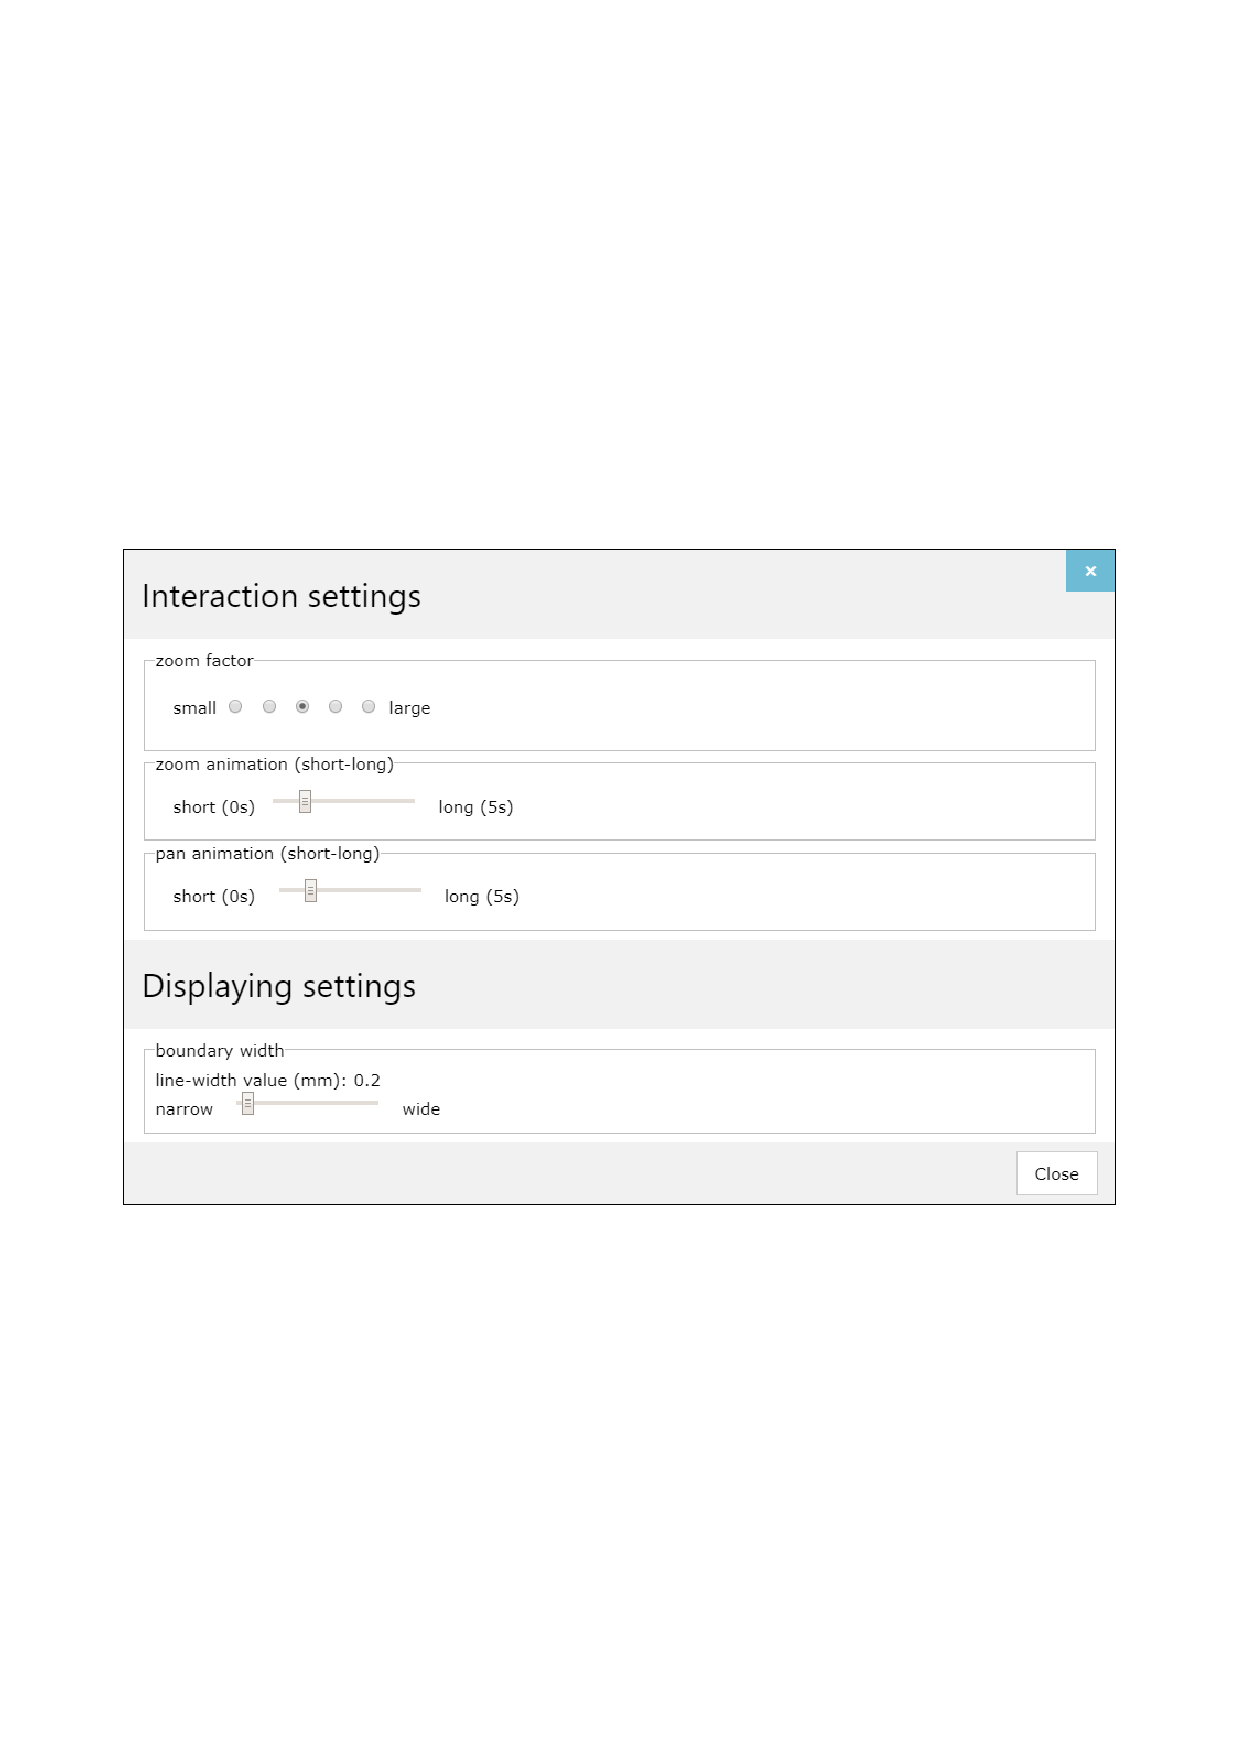
\includegraphics[page=1,scale=0.8]{case_study}
\caption{An example of our web map,
    where parallel parameter~$r_\mathrm{parallel}= 0.01$.}
\label{fig:web_map}
\end{figure}



In the following, we show some results for the case of 
parallel parameter~$r_\mathrm{parallel}= 0.01$.
The content of the JSON file is 
\begin{verbatim}
                {
                    "face_num": 13238,
                    "parallel_param": 0.01,                    
                    "eventdiff_repetition": [[0, 544]]
                }
\end{verbatim}
According to entry ``eventdiff\_repetition'',
there are~$544$ steps in total, 
which can be computed by summing up the second values in all the inner brackets.
There is only one pair of inner brackets in the list
when parallel parameter~$r_\mathrm{parallel}= 0.01$,
which shows that the compression strategy illustrated in
\sect\ref{sec:snap} is very efficient.
However, the strategy is not always that efficient;
when~$r_\mathrm{parallel}= 0.1$, for example,
there are many pairs of values in the list
(see $L_\mathrm{diff\_rep}$ in \tbl\ref{tbl:parallel_param_comparison}).
%
As explained in \sect\ref{sec:greedy_algo}, 
for each merging step we iteratively select the least important area 
and its most compatible neighbor to define a merging event; 
then, we block the neighbors of the two areas.
Sometimes, a least important area is already blocked 
because of the previously found events.
This situation happens~$3{,}216$ times in total for all the steps
(see column~$n_\mathrm{blocked}$ of \tbl\ref{tbl:parallel_param_comparison}).
%
Sometimes, although a least important area is free, 
its most compatible neighbor has been blocked 
because of the previously found events.
This case happens~$1{,}841$ times in total for all the steps
(see column~$n_\mathrm{nbr\_blocked}$ of \tbl\ref{tbl:parallel_param_comparison}).
%
More statistics of the results when 
parallel parameter~$r_\mathrm{parallel}=0.001$, $0.01$, or $0.1$ 
are shown in \tbl\ref{tbl:parallel_param_comparison}.
Apparently, when merging a larger proportion of 
the area objects, we encounter more cases of the areas blocked.

\begin{table}[tb]
\centering
\caption{The statistics when different parallel parameters area used 
(\ie~$r_\mathrm{parallel}=0.001$, $0.01$, or $0.1$).}
\begin{tabular}{rrrr}
\hline
$r_\mathrm{parallel}$   & $L_\mathrm{diff\_rep}$        & $n_\mathrm{blocked}$  & $n_\mathrm{nbr\_blocked}$ \\ \hline
0.001                   & [[0, 3195]]                   &       228             &       72                  \\
0.01                    & [[0, 544]]                    &   3{,}216             &  1{,}841                  \\
0.1                     & $L_{\mathrm{diff\_rep}, 0.1}$ & 105{,}980             & 38{,}232                  \\ \hline 
\end{tabular}
%\begin{tabular}{cccc}
%\hline
%$r_\mathrm{parallel}$ & 0.001       & 0.01          & 0.1    \\ \hline
%eventdiff\_repetition & [[0, 3195]] & [[0, 544]]    & $L_{\mathrm{diff\_rep}, 0.1}$   \\
%least face blocked    & 228            & 3{,}216         & 105{,}980       \\
%best neighbor blocked & 72            & 1{,}841        & 38{,}232 \\ \hline 
%\end{tabular}
\begin{Verbatim}[fontfamily=normal,commandchars=\\\{\},
codes={\catcode`$=3\catcode`^=7\catcode`_=8}]
$L_{\mathrm{diff\_rep},0.1}$ = [[51, 1], [138, 1], [152, 1], [200, 1], [205, 1], [181, 1], [198, 1], [167, 1], [173, 1], [165, 1], 
[153, 1], [143, 1], [140, 1], [127, 1], [125, 1], [108, 1], [103, 1], [92, 2], [84, 1], [79, 1], [74, 1], [68, 1], 
[60, 1], [54, 1], [46, 1], [50, 1], [48, 1], [45, 1], [39, 1], [44, 1], [37, 1], [36, 1], [32, 1], [30, 1], [26, 1], 
[28, 1], [21, 2], [18, 1], [20, 1], [16, 1], [12, 1], [13, 1], [8, 1], [12, 2], [6, 1], [12, 1], [11, 1], [8, 1], [7, 1], 
[6, 1], [7, 1], [4, 1], [5, 1], [4, 1], [5, 2], [7, 1], [5, 1], [4, 1], [5, 1], [3, 1], [4, 1], [3, 3], [2, 2], [1, 2], [2, 1], 
[1, 2], [2, 1], [1, 3], [0, 2], [1, 2], [0, 14]]
\end{Verbatim}
%\fvset{gobble=2}
%\begin{Verbatim}[fontfamily=normal,frame=single,
%label=$L_{\mathrm{diff\_rep}, 0.1}$]
%   [[51, 1], [138, 1], [152, 1], [200, 1], [205, 1], [181, 1], [198, 1], [167, 1], [173, 1], [165, 1], 
%    [153, 1], [143, 1], [140, 1], [127, 1], [125, 1], [108, 1], [103, 1], [92, 2], [84, 1], [79, 1], [74, 1], [68, 1], 
%    [60, 1], [54, 1], [46, 1], [50, 1], [48, 1], [45, 1], [39, 1], [44, 1], [37, 1], [36, 1], [32, 1], [30, 1], [26, 1], 
%    [28, 1], [21, 2], [18, 1], [20, 1], [16, 1], [12, 1], [13, 1], [8, 1], [12, 2], [6, 1], [12, 1], [11, 1], [8, 1], [7, 1], 
%    [6, 1], [7, 1], [4, 1], [5, 1], [4, 1], [5, 2], [7, 1], [5, 1], [4, 1], [5, 1], [3, 1], [4, 1], [3, 3], [2, 2], [1, 2], [2, 1], 
%    [1, 2], [2, 1], [1, 3], [0, 2], [1, 2], [0, 14]]
%\end{Verbatim}
\label{tbl:parallel_param_comparison}
\end{table}







When zooming on our web maps with different parallel parameters,
we observed that the impressions of the maps 
based on single-event merging and based on parallel parameter~$r_\mathrm{parallel}= 0.001$ are almost the same.
The reason is that the smooth merging happens too fast,
and we cannot really see the animation of the expansion.
We get the feeling of smooth merging when~$r_\mathrm{parallel}= 0.01$.
when~$r_\mathrm{parallel}= 0.1$, the smooth merging is already obvious.
Of course, the animation speed also depends on how much we want to zoom
when we scroll the mouse wheel (zoom factor) 
and depends on the specified animation duration (zoom animation);
see \fig\ref{fig:interaction_settings}.


\begin{figure}[tb]
\centering
\includegraphics[page=2,scale=0.7]{case_study}
\caption{Our panel of settings. 
Among others, one can set how much to zoom when scrolling the mouse wheel 
and set the animation duration of the zooming.}
\label{fig:interaction_settings}
\end{figure}

When parallel parameter~$r_\mathrm{parallel}$ is set to~$0.1$,
we notice a problem in the northeast corner of the map.
That is, some small areas stays until the scale is very small
while they should be merged much earlier.
This is due to the fact that 
there are many buildings in the northeast corner of the map.
When the buildings share the same surrounding area,
they become holes of the polygon.
In each step, only one of the buildings will be merged into the surrounding area
because an area is allowed to merge with only one area in each step.
In the meantime, the areas at other places of the map merge relatively fast
because we allow $10\%$ of the areas to be merged in each step.
To fix the problem, we should allow a surrounding area 
to merge with many of its holes in a single step.






\section{Concluding Remarks}
\label{sec:concluding_remarks}

\subsection{Conclusion}
%For the first time, 
This paper parallels generalization operations,
using the merging operation as a case study. 
This paper develops a greedy algorithm to find parallel events of 
merging area objects.
Then, the parallel events are integrated into 
the tGAP and the SSC so that the merging animations can be nicely visualized.
This paper also proposes a strategy 
to concisely store the number of merging events for all the steps.
To guarantee that the merging animations always complete for zooming, 
we manage to snap zooming operations to existing states.
Our case study shows that 
our approach provides smooth merging for zooming.


\subsection{Future Work}

Many topics related to this research need to be investigated further.
\fig\ref{fig:smooth_merging} shows our current solution of
gradually expanding an area over the other area.
In order to make the expansion even smoother,
we would like to implement the way of expanding
shown in \fig\ref{fig:smooth_merging_future}.

\begin{figure}[tb]
\centering
\includegraphics[page=3]{smooth_merging}
\caption{A smooth way of merging two areas, 
    which we would like to achieve in future.
    The larger area expands over the smaller one.
    At the same time, 
    the smaller area gradually adapt to the color of the larger one,
    and the common boundary becomes thinner and thinner.}
\label{fig:smooth_merging_future}
\end{figure}

This paper used a greedy algorithm 
to find parallel merging events for each step.
Alternatively, it is also possible to define merging steps 
by selecting and combining some single-event steps of a sequence found 
by some existing methods
(\eg~the greedy algorithm of \citet{vanOosterom2005}
or the \Astar algorithm of \citet[\chap2]{Peng2019Thesis}).

Currently, the merging events distribute randomly on a map.
If we are unlucky, there may be a lot of events happening in the screen 
for a time duration,
which are difficult for us to follow;
for another time duration, there may be no event happening in the screen at all.
A good strategy is to evenly distribute the merging events for each step, 
then the workload for us to follow the events is stable during the zooming.
To this end, we could divide a map into many regions using road network.
Then, we could find a certain number of events in each of the regions according to
the regions' sizes.


Our current event consists of only the merging operation,
it is also necessary to involve split operation
because sometimes a merging operation results in an unnatural area.
For example, it is weird to merge a long and thin area 
with one of the areas that are along it
\citep[see][]{Haunert2008Skeleton}.
Therefore, such kind of long and thin areas should be
split into several parts first.
We may integrate a split method based on the straight skeleton
\citep{Haunert2008Skeleton}
or the skeleton based on constrained Delaunay triangulation
\citep{Meijers2016Split}.
In order to apply appropriate generalization operators
for a certain scale,
we also need to extend and implement the framework 
to guide our generalization choices
\citep{Meijers2018Framework}.

To avoid clutter of vertices for zooming out, 
we also need to simplify the boundaries of the areas.
Many existing methods could be integrated into our parallel paradigm.
\citet{Meijers2011LineSimp} proposed a method 
to simplify the boundaries parallelly. 
Moreover, their results are topologically safe. 
Another choice would be the method of \citet{ImaiIri1988},
which is able to minimize the number of vertices 
for a given error threshold.
One more choice would be to construct compatible triangulations 
\citep[see][\chap3]{Peng2019Thesis}
for the two levels of land-cover maps.
In the SSC, we could build some tilted walls 
to connect the two levels of compatible triangulations.
When we slice this SSC to animate a zooming action,
the boundaries of the areas are morphed 
between a detailed representation and a coarse representation.
We can imagine that it is challenging to build the tilted walls.

This paper develops technique for smooth zooming based on parallel merging,
and we hope that it allows map users to follow the zooming more easily.
A future work is to investigate 
how much map users benefit from our technique.
We will conduct some usability tests based on the experience of
\citet[\sect6.7]{Suba2017Thesis} and \citet{Midtbo2007}.




%When we remove a triangle by slicing the SSC, 
%we may want to keep three vertices of the triangle 
%instead of making four vertices.
%In this case, the polyhedron (with five faces) should have curly edges,
%which is also known as a \emph{curved polyhedron}.
%The slopes of curly edges need to be studied.








%Some research questions are as follows.
%What aspects should we optimize 
%(\eg~minimizing the number of merging events or 
%assigning similar numbers of merging steps to each event)?
%What algorithm should we use 
%(\eg~dynamic programming, \Astar, or integer linear programming)?
%How much time is gained for users to observe the merging steps on the screen?
%How to store the parallel merging steps?






%\begin{figure}[tb]
%%\centering
%%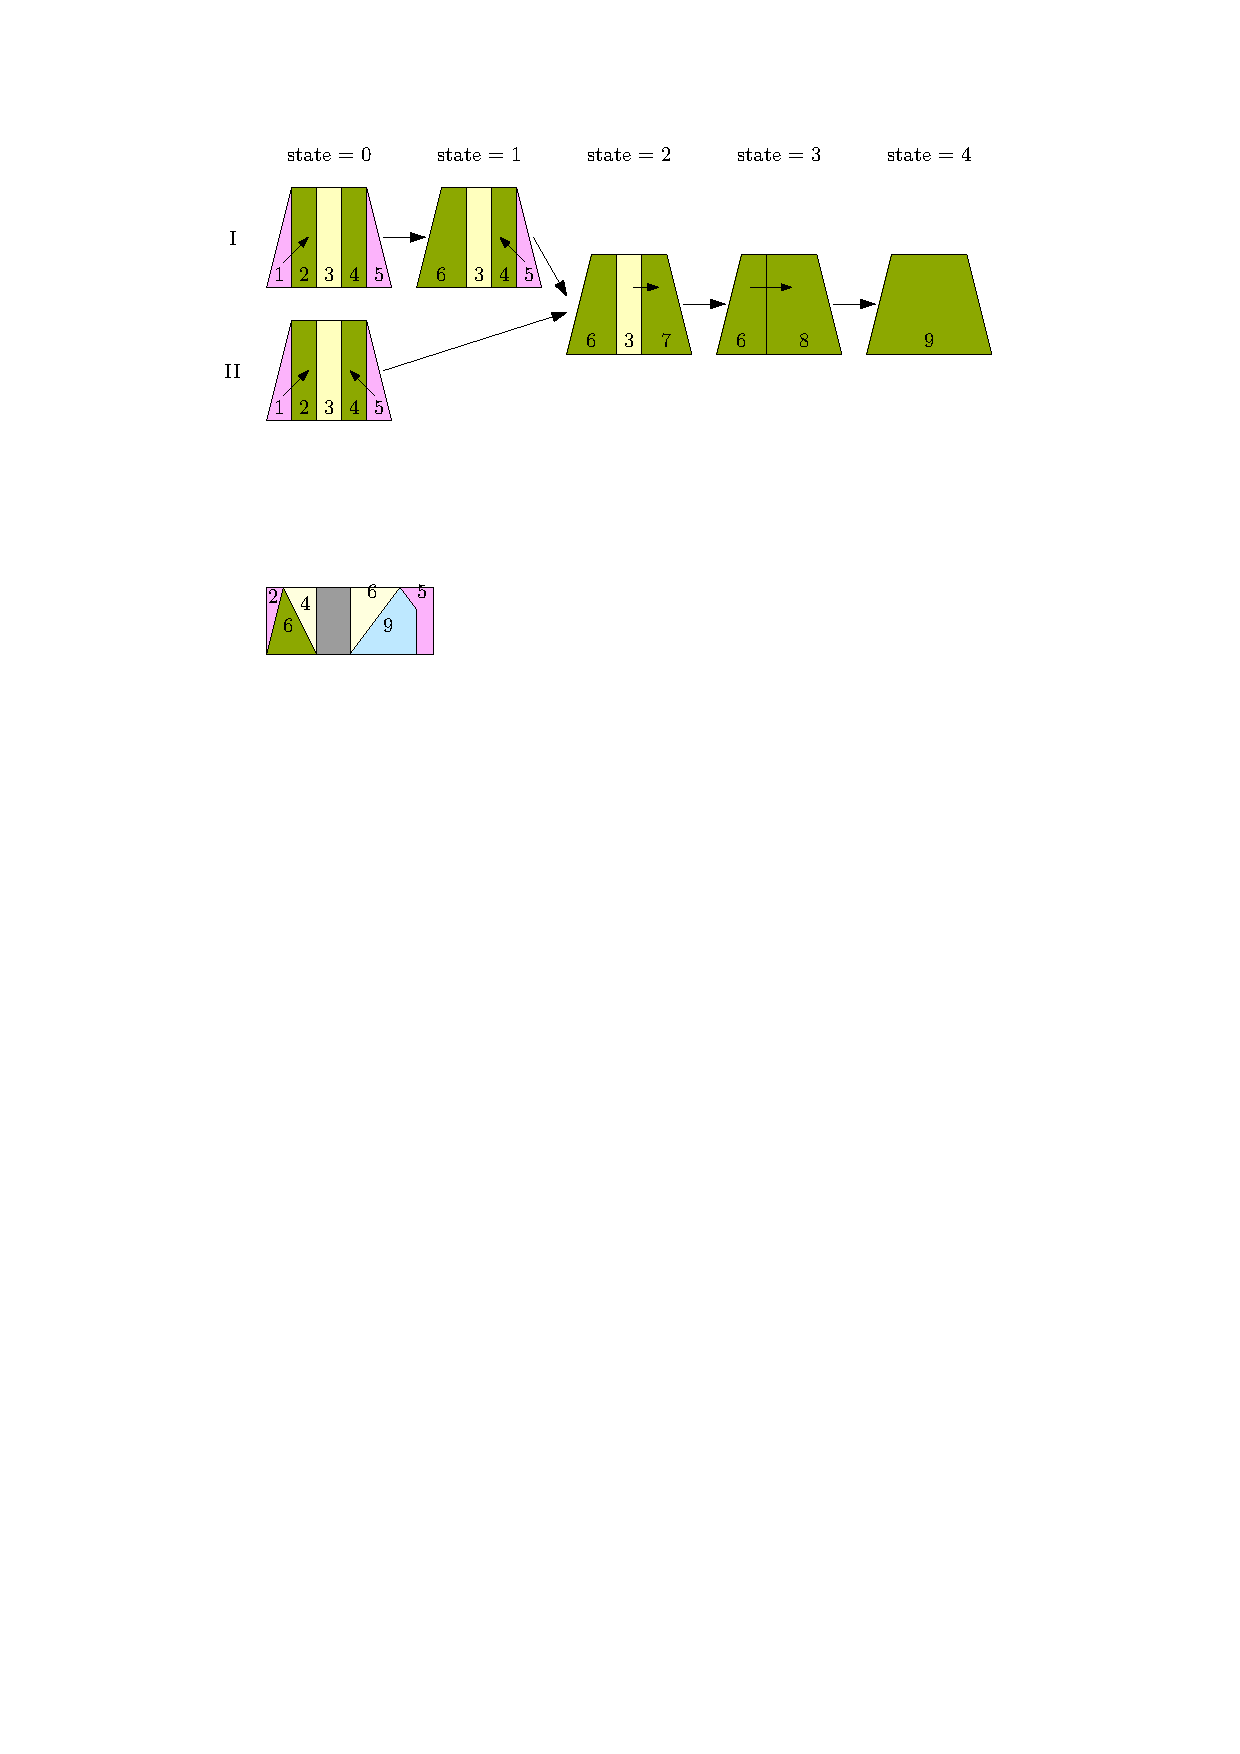
\includegraphics[page=1]{single_parallel_comparison}
%%\caption{Merging one pair of areas in each step (sequence~I), 
%%    and merging two pairs of areas parallelly (sequence~II).
%%    The arrows in the subfigures indicate merging events.}
%%\label{fig:face_tgap}
%%\vspace{8mm} %for some reason, the space below the caption is not enough
%%
%%
%%
%\captionsetup*{type=table} %*: suppress warning "The caption type was already set to figure"
%\parbox{.49\linewidth}{
%\caption{Some columns of the face table of the single-event merging steps
%    (sequence~I of \fig\ref{fig:face_tgap}).}
%\label{tbl:face_tgap}
%\centering
%\begin{tabular}{ccc}
%\hline
%face\_id & state\_low   & state\_high \\ \hline
%1       &     0         &     1       \\
%2       &     0         &     1       \\
%3       &     0         &     2       \\ 
%4       &     0         &     5       \\
%5       &     0         &     4       \\
%6       &     0         &     3       \\         
%7       &     0         &     3       \\
%8       &     1         &     2       \\
%9       &     2         &     6       \\         
%10      &     3         &     4       \\
%11      &     4         &     5       \\ 
%12      &     5         &     6       \\ 
%13      &     6         &    ---      \\ \hline
%\end{tabular}
%%\begin{tabular}{ccccc}
%%\hline
%%face\_id & state\_low   & state\_high & if\_winner  & parent\_face\_id  \\ \hline
%%1       &     0         &     1       &     0       &     8          \\
%%2       &     0         &     1       &     1       &     8          \\
%%3       &     0         &     2       &     0       &     9          \\ 
%%4       &     0         &     5       &     0       &     12          \\
%%5       &     0         &     4       &     0       &     11          \\
%%6       &     0         &     3       &     1       &     10          \\         
%%7       &     0         &     3       &     0       &     10          \\
%%8       &     1         &     2       &     1       &     9          \\
%%9       &     2         &     6       &     0       &     13          \\         
%%10      &     3         &     4       &     1       &     11          \\
%%11      &     4         &     5       &     1       &     12          \\ 
%%12      &     5         &     6       &     1       &     13          \\ 
%%13      &     6         & $\infty$    &     0       &     0          \\ \hline
%%\end{tabular}
%}
%%
%%
%\parbox{.49\linewidth}{
%\caption{Some columns of the face table of the parallel-event merging steps
%    (sequence~II of \fig\ref{fig:face_tgap}).}
%\label{tbl:face_tgap_parallel}
%\centering
%\begin{tabular}{ccc} %\underbar{2}
%\hline
%face\_id & state\_low   & state\_high \\ \hline
%1       &     0         &\underbar{2} \\
%2       &     0         &\underbar{2} \\
%3       &     0         &\underbar{4} \\ 
%4       &     0         &     5       \\
%5       &     0         &     4       \\
%6       &     0         &\underbar{2} \\         
%7       &     0         &\underbar{2} \\
%8       &\underbar{2}   &\underbar{4} \\
%9       &     2         &\underbar{6} \\         
%10      &\underbar{4}   &\underbar{4} \\
%11      &     4         &     5       \\ 
%12      &     5         &     6       \\ 
%13      &     6         &    ---      \\ \hline
%\end{tabular}
%}
%\vspace{8mm} %make some space
%%
%\captionsetup*{type=figure} %*: suppress warning "The caption type was already set to figure"
%%
%\begin{subfigure}[b]{0.49\textwidth}
% \centering
% \includegraphics[page=4,width=0.95\linewidth]{methodology}
% \caption{$y=x$}
% \label{fig:y equals x}
%\end{subfigure}
%\hfill
%\begin{subfigure}[b]{0.49\textwidth}
% \centering
% \includegraphics[page=5,width=0.95\linewidth]{methodology}
% \caption{$y=3sinx$}
% \label{fig:three sin x}
%\end{subfigure}
%\caption{The space-scale cubes of the two merging sequences, 
%where the vertical faces are removed 
%because they are not important for outputting a map.}
%\end{figure}






%%%%%%%%%%%%%%%%%%%%%%%%%%%%%%%%%%%%%%%%%%%
%\section{Patents}
%This section is not mandatory, but may be added if there are patents resulting from the work reported in this manuscript.
%
%%%%%%%%%%%%%%%%%%%%%%%%%%%%%%%%%%%%%%%%%%%
%\vspace{6pt} 
%
%%%%%%%%%%%%%%%%%%%%%%%%%%%%%%%%%%%%%%%%%%%
%%% optional
%%\supplementary{The following are available online at \linksupplementary{s1}, Figure S1: title, Table S1: title, Video S1: title.}
%
%% Only for the journal Methods and Protocols:
%% If you wish to submit a video article, please do so with any other supplementary material.
%% \supplementary{The following are available at \linksupplementary{s1}, Figure S1: title, Table S1: title, Video S1: title. A supporting video article is available at doi: link.}
%
%%%%%%%%%%%%%%%%%%%%%%%%%%%%%%%%%%%%%%%%%%%
%\authorcontributions{For research articles with several authors, a short paragraph specifying their individual contributions must be provided. The following statements should be used ``conceptualization, X.X. and Y.Y.; methodology, X.X.; software, X.X.; validation, X.X., Y.Y. and Z.Z.; formal analysis, X.X.; investigation, X.X.; resources, X.X.; data curation, X.X.; writing--original draft preparation, X.X.; writing--review and editing, X.X.; visualization, X.X.; supervision, X.X.; project administration, X.X.; funding acquisition, Y.Y.'', please turn to the  \href{http://img.mdpi.org/data/contributor-role-instruction.pdf}{CRediT taxonomy} for the term explanation. Authorship must be limited to those who have contributed substantially to the work reported.}
%
%%%%%%%%%%%%%%%%%%%%%%%%%%%%%%%%%%%%%%%%%%%
%\funding{Please add: ``This research received no external funding'' or ``This research was funded by NAME OF FUNDER grant number XXX.'' and  and ``The APC was funded by XXX''. Check carefully that the details given are accurate and use the standard spelling of funding agency names at \url{https://search.crossref.org/funding}, any errors may affect your future funding.}
%
%%%%%%%%%%%%%%%%%%%%%%%%%%%%%%%%%%%%%%%%%%%
%\acknowledgments{In this section you can acknowledge any support given which is not covered by the author contribution or funding sections. This may include administrative and technical support, or donations in kind (e.g., materials used for experiments).}
%
%%%%%%%%%%%%%%%%%%%%%%%%%%%%%%%%%%%%%%%%%%%
%\conflictsofinterest{Declare conflicts of interest or state ``The authors declare no conflict of interest.'' Authors must identify and declare any personal circumstances or interest that may be perceived as inappropriately influencing the representation or interpretation of reported research results. Any role of the funders in the design of the study; in the collection, analyses or interpretation of data; in the writing of the manuscript, or in the decision to publish the results must be declared in this section. If there is no role, please state ``The funders had no role in the design of the study; in the collection, analyses, or interpretation of data; in the writing of the manuscript, or in the decision to publish the results''.} 
%
%%%%%%%%%%%%%%%%%%%%%%%%%%%%%%%%%%%%%%%%%%%
%%% optional
%\abbreviations{The following abbreviations are used in this manuscript:\\
%
%\noindent 
%\begin{tabular}{@{}ll}
%MDPI & Multidisciplinary Digital Publishing Institute\\
%DOAJ & Directory of open access journals\\
%TLA & Three letter acronym\\
%LD & linear dichroism
%\end{tabular}}
%
%%%%%%%%%%%%%%%%%%%%%%%%%%%%%%%%%%%%%%%%%%%
%%% optional
%\appendixtitles{no} %Leave argument "no" if all appendix headings stay EMPTY (then no dot is printed after "Appendix A"). If the appendix sections contain a heading then change the argument to "yes".
%\appendix
%\section{}
%\unskip
%\subsection{}
%The appendix is an optional section that can contain details and data supplemental to the main text. For example, explanations of experimental details that would disrupt the flow of the main text, but nonetheless remain crucial to understanding and reproducing the research shown; figures of replicates for experiments of which representative data is shown in the main text can be added here if brief, or as Supplementary data. Mathematical proofs of results not central to the paper can be added as an appendix.
%
%\section{}
%All appendix sections must be cited in the main text. In the appendixes, Figures, Tables, etc. should be labeled starting with `A', e.g., Figure A1, Figure A2, etc. 

%%%%%%%%%%%%%%%%%%%%%%%%%%%%%%%%%%%%%%%%%%
% Citations and References in Supplementary files are permitted provided that they also appear in the reference list here. 

%=====================================
% References, variant A: internal bibliography
%=====================================
%\reftitle{References}
%\begin{thebibliography}{999}
%% Reference 1
%\bibitem[Author1(year)]{ref-journal}
%Author1, T. The title of the cited article. {\em Journal Abbreviation} {\bf 2008}, {\em 10}, 142--149.
%% Reference 2
%\bibitem[Author2(year)]{ref-book}
%Author2, L. The title of the cited contribution. In {\em The Book Title}; Editor1, F., Editor2, A., Eds.; Publishing House: City, Country, 2007; pp. 32--58.
%\end{thebibliography}
\bibliography{Reference/BibReference}

% The following MDPI journals use author-date citation: Arts, Econometrics, Economies, Genealogy, Humanities, IJFS, JRFM, Laws, Religions, Risks, Social Sciences. For those journals, please follow the formatting guidelines on http://www.mdpi.com/authors/references
% To cite two works by the same author: \citeauthor{ref-journal-1a} (\citeyear{ref-journal-1a}, \citeyear{ref-journal-1b}). This produces: Whittaker (1967, 1975)
% To cite two works by the same author with specific pages: \citeauthor{ref-journal-3a} (\citeyear{ref-journal-3a}, p. 328; \citeyear{ref-journal-3b}, p.475). This produces: Wong (1999, p. 328; 2000, p. 475)

%=====================================
% References, variant B: external bibliography
%=====================================
%\externalbibliography{yes}
%\bibliography{your_external_BibTeX_file}

%%%%%%%%%%%%%%%%%%%%%%%%%%%%%%%%%%%%%%%%%%
%% optional
%\sampleavailability{Samples of the compounds ...... are available from the authors.}

%% for journal Sci
%\reviewreports{\\
%Reviewer 1 comments and authors’ response\\
%Reviewer 2 comments and authors’ response\\
%Reviewer 3 comments and authors’ response
%}








%%%%%%%%%%%%%%%%%%%%%%%%%%%%%%%%%%%%%%%%%%
\end{document}

